% defer/rcuusage.tex

\subsection{RCU Usage}
\label{sec:defer:RCU Usage}
\OriginallyPublished{Section}{sec:defer:RCU Usage}{RCU Usage}{Linux Weekly News}{PaulEMcKenney2008WhatIsRCUUsage}

\begin{table}[tb]
\renewcommand*{\arraystretch}{1.2}
\centering
\small
\begin{tabular}{ll}
\toprule
Mechanism RCU Replaces & Section \\
\midrule
Reader-writer locking &
	Section~\ref{sec:defer:RCU is a Reader-Writer Lock Replacement} \\
Restricted reference-counting mechanism &
	Section~\ref{sec:defer:RCU is a Restricted Reference-Counting Mechanism} \\
Bulk reference-counting mechanism &
	Section~\ref{sec:defer:RCU is a Bulk Reference-Counting Mechanism} \\
Poor man's garbage collector &
	Section~\ref{sec:defer:RCU is a Poor Man's Garbage Collector} \\
Existence Guarantees &
	Section~\ref{sec:defer:RCU is a Way of Providing Existence Guarantees} \\
Type-Safe Memory &
	Section~\ref{sec:defer:RCU is a Way of Providing Type-Safe Memory} \\
Wait for things to finish &
	Section~\ref{sec:defer:RCU is a Way of Waiting for Things to Finish} \\
\bottomrule
\end{tabular}
\caption{RCU Usage}
\label{tab:defer:RCU Usage}
\end{table}

이 섹션은 ``RCU 는 무엇인가?'' 라는 질문에 대해 RCU 가 사용될 수 있는 경우에
대한 관점에서 답변해 보겠습니다.
RCU 는 존재하는 메커니즘 중 일부를 대체하는데 용도로 가장 자주 사용되기 때문에,
Table~\ref{tab:defer:RCU Usage} 에 보여진 것처럼 그런 메커니즘들과의 관계에
대한 점을 중심적으로 알아보겠습니다.
이 테이블에 나열된 섹션들을 뒤이어서, Section~\ref{sec:defer:RCU Usage Summary}
에서는 요약을 제공합니다.
\iffalse

This section answers the question ``What is RCU?'' from the viewpoint
of the uses to which RCU can be put.
Because RCU is most frequently used to replace some existing mechanism,
we look at it primarily in terms of its relationship to such mechanisms,
as listed in Table~\ref{tab:defer:RCU Usage}.
Following the sections listed in this table,
Section~\ref{sec:defer:RCU Usage Summary} provides a summary.
\fi

\subsubsection{RCU for Pre-BSD Routing}
\label{sec:defer:RCU for Pre-BSD Routing}

\begin{listing}[tbp]
{ \scriptsize
\begin{verbbox}
 1 struct route_entry {
 2   struct rcu_head rh;
 3   struct cds_list_head re_next;
 4   unsigned long addr;
 5   unsigned long iface;
 6   int re_freed;
 7 };
 8 CDS_LIST_HEAD(route_list);
 9 DEFINE_SPINLOCK(routelock);
10
11 unsigned long route_lookup(unsigned long addr)
12 {
13   struct route_entry *rep;
14   unsigned long ret;
15
16   rcu_read_lock();
17   cds_list_for_each_entry_rcu(rep, &route_list,
18                               re_next) {
19     if (rep->addr == addr) {
20       ret = rep->iface;
21       if (READ_ONCE(rep->re_freed))
22         abort();
23       rcu_read_unlock();
24       return ret;
25     }
26   }
27   rcu_read_unlock();
28   return ULONG_MAX;
29 }
\end{verbbox}
}
\centering
\theverbbox
\caption{RCU Pre-BSD Routing Table Lookup}
\label{lst:defer:RCU Pre-BSD Routing Table Lookup}
\end{listing}

\begin{listing}[tbp]
{ \scriptsize
\begin{verbbox}
 1 int route_add(unsigned long addr,
 2               unsigned long interface)
 3 {
 4   struct route_entry *rep;
 5
 6   rep = malloc(sizeof(*rep));
 7   if (!rep)
 8     return -ENOMEM;
 9   rep->addr = addr;
10   rep->iface = interface;
11   rep->re_freed = 0;
12   spin_lock(&routelock);
13   cds_list_add_rcu(&rep->re_next, &route_list);
14   spin_unlock(&routelock);
15   return 0;
16 }
17
18 static void route_cb(struct rcu_head *rhp)
19 {
20   struct route_entry *rep;
21
22   rep = container_of(rhp, struct route_entry, rh);
23   WRITE_ONCE(rep->re_freed, 1);
24   free(rep);
25 }
26
27 int route_del(unsigned long addr)
28 {
29   struct route_entry *rep;
30
31   spin_lock(&routelock);
32   cds_list_for_each_entry(rep, &route_list,
33                           re_next) {
34     if (rep->addr == addr) {
35       cds_list_del_rcu(&rep->re_next);
36       spin_unlock(&routelock);
37       call_rcu(&rep->rh, route_cb);
38       return 0;
39     }
40   }
41   spin_unlock(&routelock);
42   return -ENOENT;
43 }
\end{verbbox}
}
\centering
\theverbbox
\caption{RCU Pre-BSD Routing Table Add/Delete}
\label{lst:defer:RCU Pre-BSD Routing Table Add/Delete}
\end{listing}

Listing~\ref{lst:defer:RCU Pre-BSD Routing Table Lookup}
와~\ref{lst:defer:RCU Pre-BSD Routing Table Add/Delete}
는 RCU 로 보호되는 Pre-BSD 라우팅 테이블을 위한 코드를 보이고 있습니다
(\path{route_rcu.c}).
앞의 것은 데이터 구조들과 \co{route_lookup()} 을, 뒤의 것은 \co{route_add()} 와
\co{route_del()} 을 위한 코드입니다.
\iffalse

Listings~\ref{lst:defer:RCU Pre-BSD Routing Table Lookup}
and~\ref{lst:defer:RCU Pre-BSD Routing Table Add/Delete}
show code for an RCU-protected Pre-BSD routing table
(\path{route_rcu.c}).
The former shows data structures and \co{route_lookup()},
and the latter shows \co{route_add()} and \co{route_del()}.
\fi

Listing~\ref{lst:defer:RCU Pre-BSD Routing Table Lookup} 에서, line~2 는 RCU
reclamation 에 사용되는 \co{->rh} 필드를 보이고, line~6 는 해제 후 사용 검사를
위한 \co{->re_freed} 필드를 보이며, line~16, 17, 23, 그리고~27 은 RCU read-side
보호 코드를 보이고, line~21 과~22 에서 해제 후 사용 여부 검사를 합니다.
Listing~\ref{lst:defer:RCU Pre-BSD Routing Table Add/Delete} 에서, line~12, 14,
31, 36, 그리고~41 에서 update-side 락킹을 하며, line~13 과~35 에서 RCU
update-side 보호를 하고, line~37 에서 grace period 가 하나 지나간 후에
\co{route_cb()} 를 호출되게 하고, line~18-25 에서 \co{route_cb()} 를
정의합니다.
이는 똑바로 동작하는 구현을 위해 추가되는 최소한의 코드입니다.
\iffalse

In Listing~\ref{lst:defer:RCU Pre-BSD Routing Table Lookup},
line~2 adds the \co{->rh} field used by RCU reclamation,
line~6 adds the \co{->re_freed} use-after-free-check field,
lines~16, 17, 23, and~27 add RCU read-side protection,
and lines~21 and~22 add the use-after-free check.
In Listing~\ref{lst:defer:RCU Pre-BSD Routing Table Add/Delete},
lines~12, 14, 31, 36, and~41 add update-side locking,
lines~13 and~35 add RCU update-side protection,
line~37 causes \co{route_cb()} to be invoked after a grace period elapses,
and lines~18-25 define \co{route_cb()}.
This is minimal added code for a working concurrent implementation.
\fi

\begin{figure}[tb]
\centering
\resizebox{2.5in}{!}{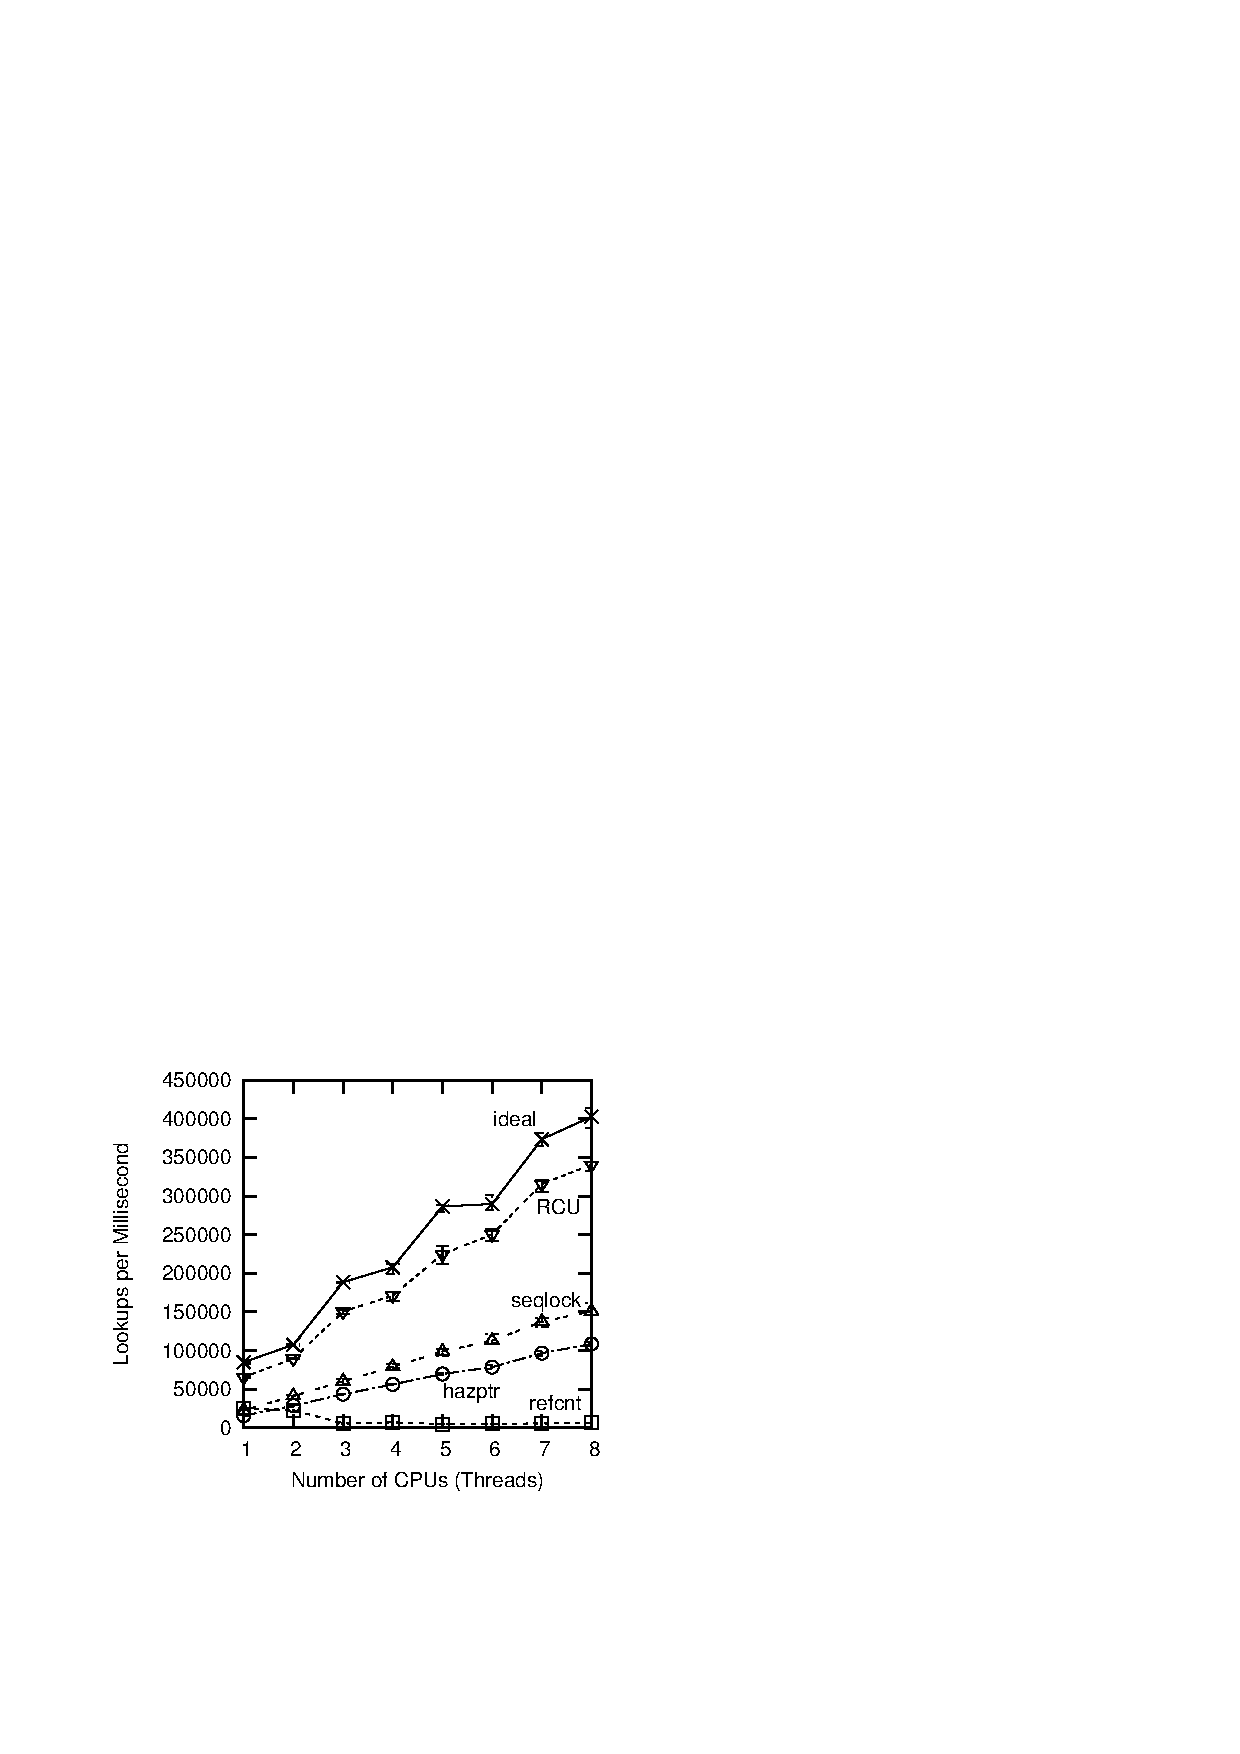
\includegraphics{CodeSamples/defer/perf-rcu}}
\caption{Pre-BSD Routing Table Protected by RCU}
\label{fig:defer:Pre-BSD Routing Table Protected by RCU}
\end{figure}

Figure~\ref{fig:defer:Pre-BSD Routing Table Protected by RCU}
는 read-only 워크로드에서의 성능을 보입니다.
RCU 는 상당히 잘 확장되어서, 이상적 성능에 가까운 성능을 보입니다.
하지만, 이 데이터는 userspace RCU 의 \co{RCU_SIGNAL} 사용
버전~\cite{MathieuDesnoyers2009URCU,PaulMcKenney2013LWNURCU} 을 사용해서 생성된
것으로, \co{rcu_read_lock()} 과 \co{rcu_read_unlock()} 이 약간의 코드를
생성합니다.
\co{rcu_read_lock()} 과 \co{rcu_read_unlock()} 에 아무 코드도 생성하지 않는
QSBR 버전의 RCU 를 사용한다면 어떻게 될까요?
(Section~\ref{sec:defer:Introduction to RCU} 를 참고하고, RCU QSBR 에 대한
논의를 위해선
Figure~\ref{fig:defer:RCU QSBR: Waiting for Pre-Existing Readers} 를
참고하세요.)
\iffalse

Figure~\ref{fig:defer:Pre-BSD Routing Table Protected by RCU}
shows the performance on the read-only workload.
RCU scales quite well, and offers nearly ideal performance.
However, this data was generated using the \co{RCU_SIGNAL}
flavor of userspace
RCU~\cite{MathieuDesnoyers2009URCU,PaulMcKenney2013LWNURCU},
for which \co{rcu_read_lock()} and \co{rcu_read_unlock()}
generate a small amount of code.
What happens for the QSBR flavor of RCU, which generates no code at all
for \co{rcu_read_lock()} and \co{rcu_read_unlock()}?
(See Section~\ref{sec:defer:Introduction to RCU},
and especially
Figure~\ref{fig:defer:RCU QSBR: Waiting for Pre-Existing Readers},
for a discussion of RCU QSBR.)
\fi

그에 대한 답이 RCU QSBR 결과를 RCU 와 ideal 사이에 보여주는
Figure~\ref{fig:defer:Pre-BSD Routing Table Protected by RCU QSBR}
에 있습니다.
RCU QSBR 은 바랬던 대로 동기화를 아예 하지 않는, 이상적인 워크로드와 거의
동일한 성능과 확장성을 갖습니다.
\iffalse

The answer to this shown in
Figure~\ref{fig:defer:Pre-BSD Routing Table Protected by RCU QSBR},
which shows the RCU QSBR results as the trace between the RCU and
the ideal traces.
RCU QSBR's performance and scalability is very nearly that of an
ideal synchronization-free workload, as desired.
\fi

\QuickQuiz{}
	RCU QSBR 은 왜 이상적 결과와 \emph{동일한} 결과를 보이지 않는 거죠?
	\iffalse

	Why doesn't RCU QSBR give \emph{exactly} ideal results?
	\fi
\QuickQuizAnswer{
	\co{rcu_dereference()} 는 컴파일러의 최적화를 조금 제약할 수 있어서,
	아주 약간 느린 코드를 만들어낼 수 있습니다.
	이 영향은 일반적으로는 별로 심각하지 않을 것입니다만, 각각의 탐색이 약
	13~나노세컨드를 더 필요로 하게 되는데, 이는 코드 생성의 작은 차이가
	느껴지지도 못할만큼 충분히 짧은 시간입니다.
	이 차이는 약 1.5\,\% 부터 약 11.1\,\% 까지 나오는데, RCU QSBR 코드가
	``이상적인'' 코드는 할 수 없는 동시의 업데이트도 처리할 수 있다는 점을
	생각하면 상당히 작은 차이입니다.
	\iffalse

	The \co{rcu_dereference()} primitive does constrain the
	compiler's optimizations somewhat, which can result in
	slightly slower code.
	This effect would normally be insignificant, but
	each search is taking on average about 13~nanoseconds,
	which is short enough for small differences in code
	generation to make their presence felt.
	The difference ranges from about 1.5\,\% to about 11.1\,\%, which is
	quite small when you consider that the RCU QSBR code can handle
	concurrent updates and the ``ideal'' code cannot.
	\fi

	C11 \co{memory_order_consume} 로드~\cite{RichardSmith2015N4527} 가
	언젠가는 \co{rcu_dereference()} 에게 더 낮은 비용에 필요한 보호를
	해주는 날이 올 것을 기대하고 있습니다.
	\iffalse

	It is hoped that C11 \co{memory_order_consume}
	loads~\cite{RichardSmith2015N4527}
	might someday allow \co{rcu_dereference()} provide the
	needed protection at lower cost.
	\fi
} \QuickQuizEnd

\QuickQuiz{}
	RCU QSBR 의 read-side 성능이 이렇게 좋은데, 왜 다른 종류의 userspace
	RCU 를 신경써야 하죠?
	\iffalse

	Given RCU QSBR's read-side performance, why bother with any
	other flavor of userspace RCU?
	\fi
\QuickQuizAnswer{
	RCU QSBR 은 어플리케이션에게 경우에 따라서는 불가능한 제약을
	강제하는데, 예를 들어 어플리케이션 내의 각각의 모든 쓰레드가 quiescent
	state 를 정규적으로 통과해야 하는 식입니다.
	무엇보다도, 이는 RCU QSBR 이 라이브러리를 만드는 사람에게는 도움이 될
	수 없음을 의미하는데, 그런 사람들은 다른 종류의 userspace RCU를
	사용하는게 좋을 겁니다~\cite{PaulMcKenney2013LWNURCU}.
	\iffalse

	Because RCU QSBR places constraints on the overall application
	that might not be tolerable,
	for example, requiring that each and every thread in the
	application regularly pass through a quiescent state.
	Among other things, this means that RCU QSBR is not helpful
	to library writers, who might be better served by other
	flavors of userspace RCU~\cite{PaulMcKenney2013LWNURCU}.
	\fi
} \QuickQuizEnd

\begin{figure}[tb]
\centering
\resizebox{2.5in}{!}{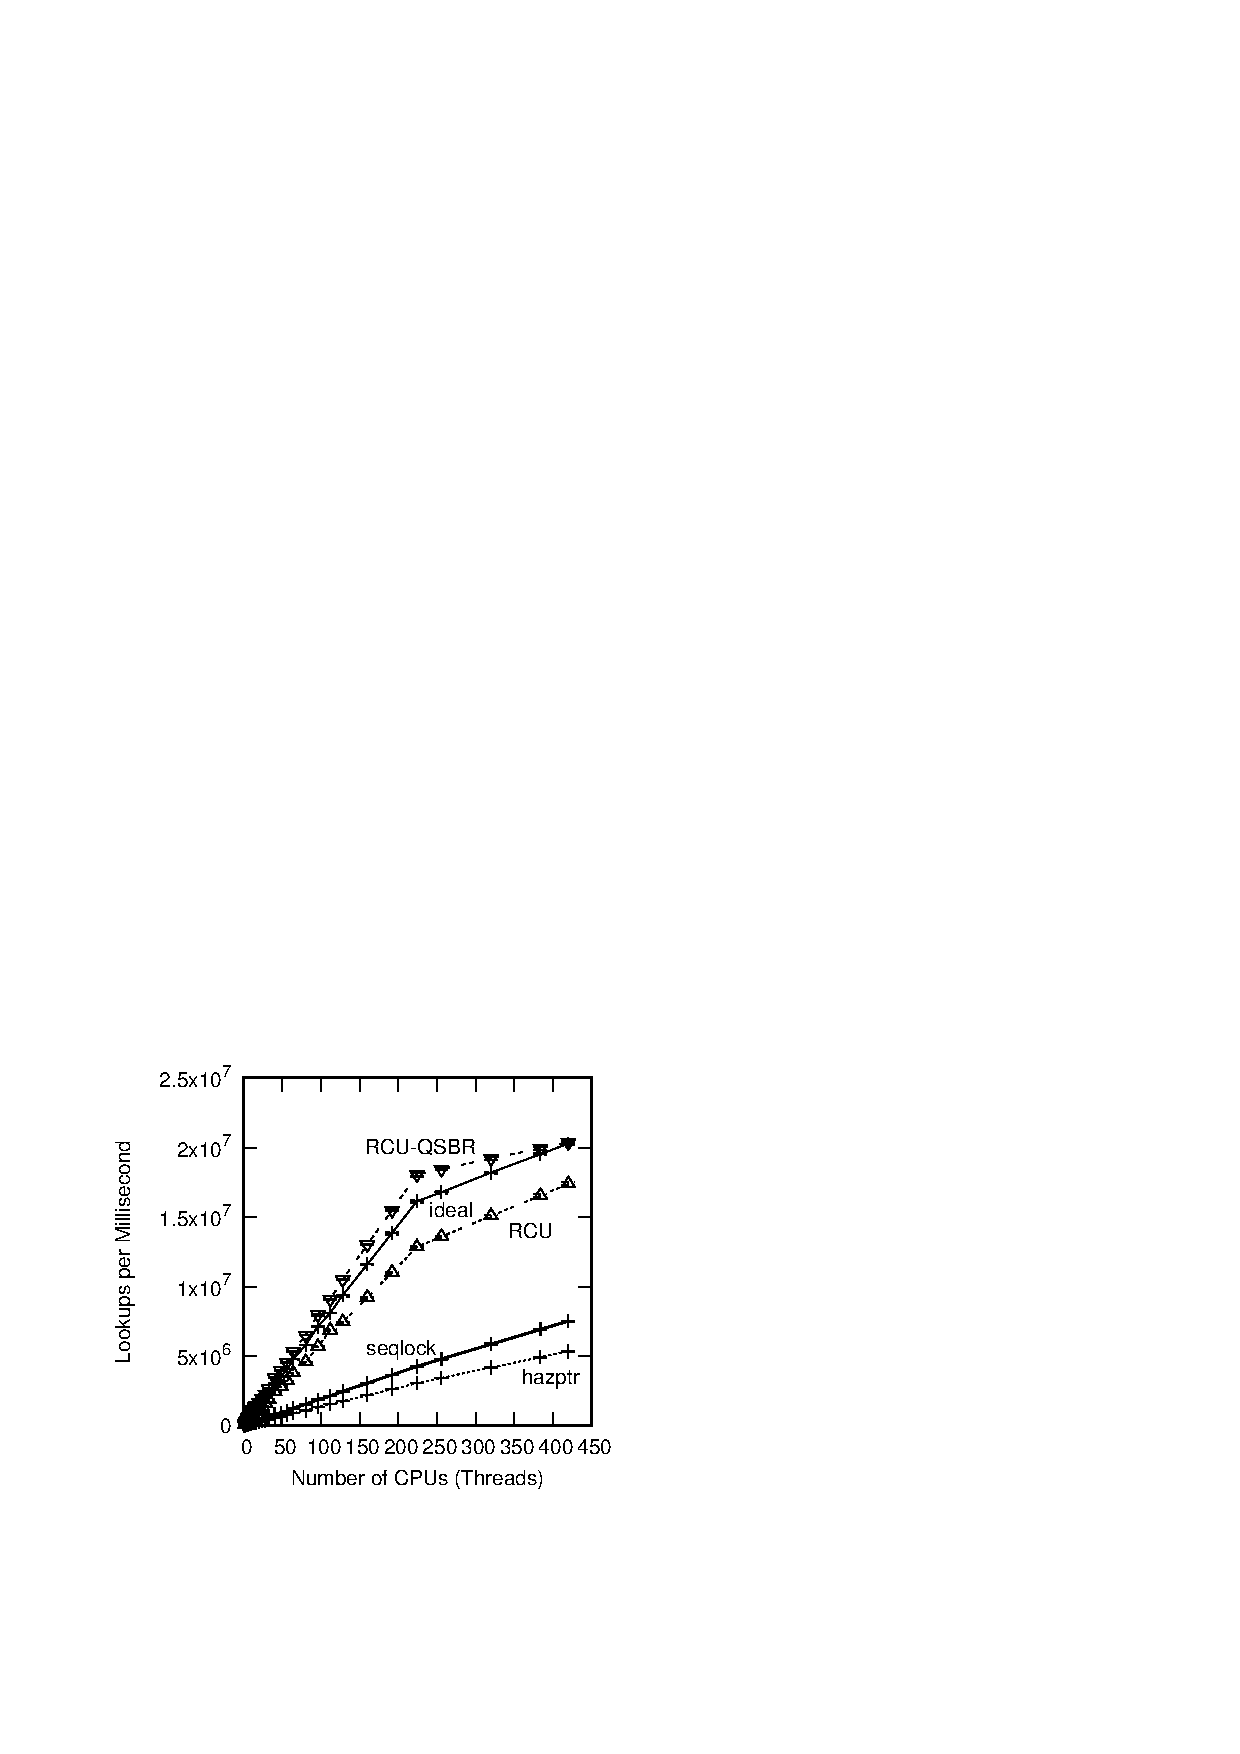
\includegraphics{CodeSamples/defer/perf-rcu-qsbr}}
\caption{Pre-BSD Routing Table Protected by RCU QSBR}
\label{fig:defer:Pre-BSD Routing Table Protected by RCU QSBR}
\end{figure}

\subsubsection{RCU is a Reader-Writer Lock Replacement}
\label{sec:defer:RCU is a Reader-Writer Lock Replacement}

리눅스 커널에서 가장 흔한 RCU 의 사용 경우는 읽기가 대부분인 상황들에서의
reader-writer 락킹의 대체입니다.
더도 아니고 덜도 아니고, 이런 RCU 의 사용은 제게는 처음부터 곧장 그래야 할
것처럼 보이진 않았는데, 실제로 저는 1990년대 초기에 범용의 RCU 구현을 만들기
전에 경량의 reader-writer 락~\cite{WilsonCHsieh92a}\footnote{
	2.4 리눅스 커널의 \co{brlock} 과 더 최신의 리눅스 커널 버전들의
	\co{lglock} 과 유사합니다}
을 구현하려 했습니다.
제가 그 경량 reader-writer 락을 위해 상상했던 모든 사용 케이스들은 대신 RCU 로
구현되었습니다.
사실, 그건 그 경량 reader-writer 락이 처음으로 사용되기보다 3년도 더 전의
일입니다.
이봐요, 과연 제가 절 바보라고 생각했을꺼라고 생각해요?
\iffalse

Perhaps the most common use of RCU within the Linux kernel is as
a replacement for reader-writer locking in read-intensive situations.
Nevertheless, this use of RCU was not immediately apparent to me
at the outset, in fact, I chose to implement a lightweight reader-writer
lock~\cite{WilsonCHsieh92a}\footnote{
	Similar to \co{brlock} in the 2.4 Linux kernel and to
	\co{lglock} in more recent Linux kernels.}
before implementing a general-purpose RCU implementation
back in the early 1990s.
Each and every one of the uses I envisioned for the lightweight reader-writer
lock was instead implemented using RCU.
In fact, it was more than
three years before the lightweight reader-writer lock saw its first use.
Boy, did I feel foolish!
\fi

RCU 와 reader-writer 락킹 사이의 핵심적인 유사점은 둘 다 병렬로 수행될 수 있는
read-side 크리티컬 섹션들을 가지고 있다는 점입니다.
사실, 어떤 경우에 있어서는, RCU API 로 연관된 reader-writer 락 API 멤버들을
기계적으로 대체하는 것이 가능합니다.
하지만 그전에, 왜 그러려 하나요?
\iffalse

The key similarity between RCU and reader-writer locking is that
both have read-side critical sections that can execute in parallel.
In fact, in some cases, it is possible to mechanically substitute RCU API
members for the corresponding reader-writer lock API members.
But first, why bother?
\fi

RCU 의 장점에는 성능, 데드락에의 내성, 그리고 리얼타임 대기시간이 포함됩니다.
물론, RCU 에도 한계가 있는데, 읽기 쓰레드와 업데이트 쓰레드가 동시에
수행될 수 없고, 낮은 중요도의 RCU 읽기 쓰레드들이 grace period 가 지나가길
기다리고 있는 높은 중요도의 쓰레드들을 블락시킬 수 있으며, 이 grace-period
대기시간은 수 밀리세컨드를 넘길 수 있다는 점등이 포함됩니다.
이런 장점들과 제한점들을 다음 섹션들에서 이야기 하겠습니다.
\iffalse

Advantages of RCU include performance,
deadlock immunity, and realtime latency.
There are, of course, limitations to RCU, including the fact that
readers and updaters run concurrently, that low-priority RCU readers
can block high-priority threads waiting for a grace period to elapse,
and that grace-period latencies can extend for many milliseconds.
These advantages and limitations are discussed in the following sections.
\fi

\paragraph{Performance}

\begin{figure}[tb]
\begin{center}
\resizebox{3in}{!}{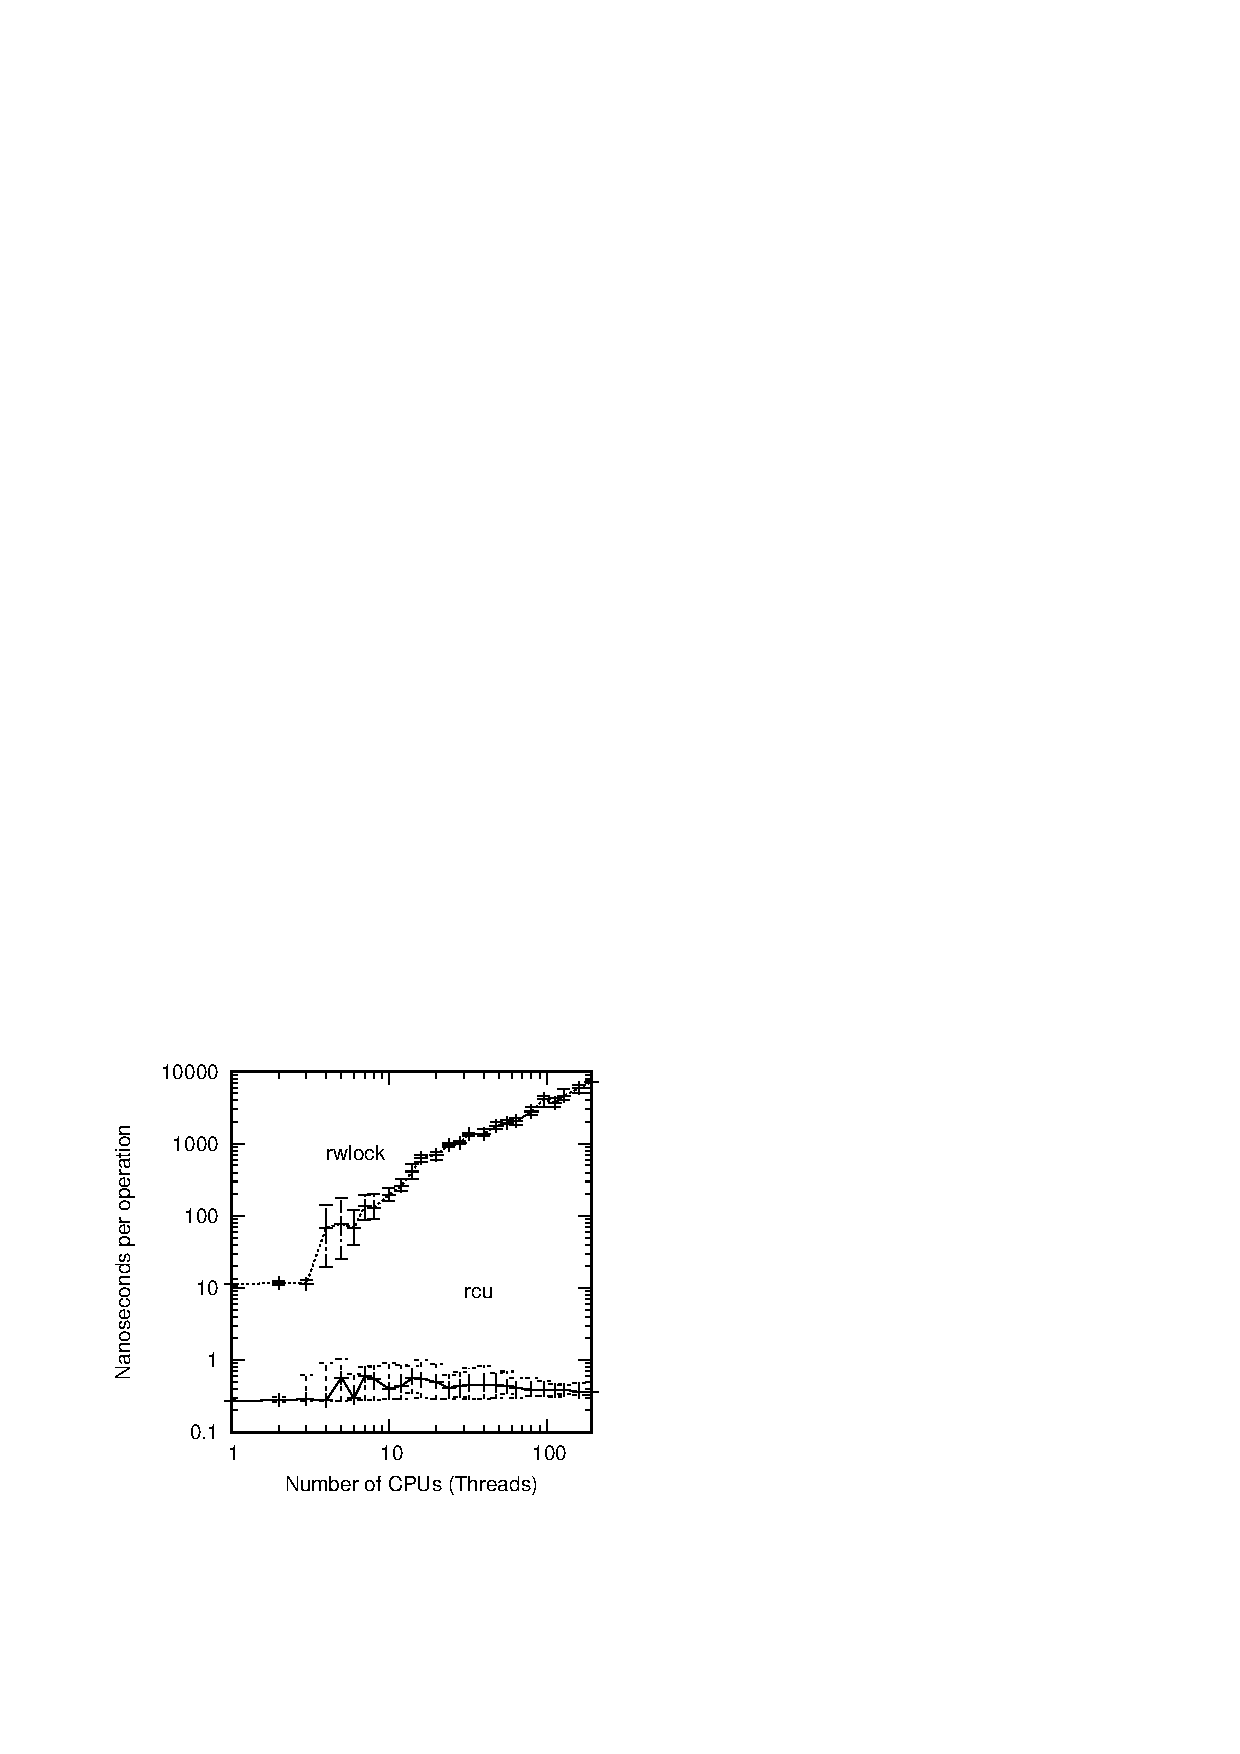
\includegraphics{defer/rwlockRCUperf}}
\end{center}
\caption{Performance Advantage of RCU Over Reader-Writer Locking}
\label{fig:defer:Performance Advantage of RCU Over Reader-Writer Locking}
\end{figure}

RCU 의 reader-writer 락킹에 대비한 읽기 작업 성능의 이점이
Figure~\ref{fig:defer:Performance Advantage of RCU Over Reader-Writer Locking}
에 그려져 있습니다.
\iffalse

The read-side performance advantages of RCU over reader-writer locking
are shown in
Figure~\ref{fig:defer:Performance Advantage of RCU Over Reader-Writer Locking}.
\fi

\QuickQuiz{}
	이게 뭐죠?
	3GHz 에서 클락 시간은 300 \emph{피코세컨드} 가 넘는데 대체 어떻게 RCU
	는 100 펜토세컨드의 오버헤드를 갖는다고 제가 믿을 수 있을 거라고
	생각하세요?
	\iffalse

	WTF?
	How the heck do you expect me to believe that RCU has a
	100-femtosecond overhead when the clock period at 3\,GHz is more than
	300 \emph{picoseconds}?
	\fi
\QuickQuizAnswer{
	먼저, 이 측정을 위해 사용된 내부의 루프가 다음과 같다고 생각해 보세요:
	\iffalse

	First, consider that the inner loop used to
	take this measurement is as follows:
	\fi

\vspace{5pt}
\begin{minipage}[t]{\columnwidth}
\scriptsize
\begin{verbatim}
  1 for (i = 0; i < CSCOUNT_SCALE; i++) {
  2   rcu_read_lock();
  3   rcu_read_unlock();
  4 }
\end{verbatim}
\end{minipage}
\vspace{5pt}

	다음으로, \co{rcu_read_lock()} 과 \co{rcu_read_unlock()} 이 실질적으로
	수행하는 코드가 다음과 같다고 생각해 봅시다: 
	\iffalse

	Next, consider the effective definitions of \co{rcu_read_lock()}
	and \co{rcu_read_unlock()}:
	\fi

\vspace{5pt}
\begin{minipage}[t]{\columnwidth}
\scriptsize
\begin{verbatim}
  1 #define rcu_read_lock()   do { } while (0)
  2 #define rcu_read_unlock() do { } while (0)
\end{verbatim}
\end{minipage}
\vspace{5pt}

	그리고 컴파일러가 이 루프를 다음과 같이 바뀌게 하는 간단한 최적화를
	한다고 생각해 보세요:
	\iffalse

	Consider also that the compiler does simple optimizations,
	allowing it to replace the loop with:
	\fi

\vspace{5pt}
\begin{minipage}[t]{\columnwidth}
\scriptsize
\begin{verbatim}
i = CSCOUNT_SCALE;
\end{verbatim}
\end{minipage}
\vspace{5pt}

	따라서 100 펨토세컨드의 ``측정'' 은 단순히 고정된 시간 측정 오버헤드를
	\co{rcu_read_lock()} 과 \co{rcu_read_unlock()} 호출을 담고 있는 루프의
	수행 횟수로 나눈 값일 뿐입니다.
	그리고 따라서, 이 측정은 실제로 에러인데, 실제로 수십수백배의
	에러율입니다.
	앞의 \co{rcu_read_lock()} 와 \co{rcu_read_unlock()} 의 정의에서 알 수
	있듯이, 실제 오버헤드는 정확히 제로입니다.

	언제까지나 100 펨토세컨드의 시간 측정이 과하게 추측된걸로 판명되는 건
	아닐 것이 분명합니다!
	\iffalse

	So the ``measurement'' of 100 femtoseconds is simply the fixed
	overhead of the timing measurements divided by the number of
	passes through the inner loop containing the calls
	to \co{rcu_read_lock()} and \co{rcu_read_unlock()}.
	And therefore, this measurement really is in error, in fact,
	in error by an arbitrary number of orders of magnitude.
	As you can see by the definition of \co{rcu_read_lock()}
	and \co{rcu_read_unlock()} above, the actual overhead
	is precisely zero.

	It certainly is not every day that a timing measurement of
	100 femtoseconds turns out to be an overestimate!
	\fi
} \QuickQuizEnd

reader-writer 락킹은 단일 CPU 위에서 RCU 보다 열배가량 느리고 16개의 CPU
위에서는 100배가 \emph{더} 느리다는 점을 알아두세요.
반면, RCU 는 상당히 잘 확장됩니다.
두 케이스 모두, 에러바들은 양쪽으로 표준편차만큼의 크기를 갖습니다.
\iffalse

Note that reader-writer locking is orders of magnitude slower than RCU
on a single CPU, and is almost two \emph{additional} orders of magnitude
slower on 16 CPUs.
In contrast, RCU scales quite well.
In both cases, the error bars span a single standard deviation in either
direction.
\fi

\begin{figure}[tb]
\begin{center}
\resizebox{3in}{!}{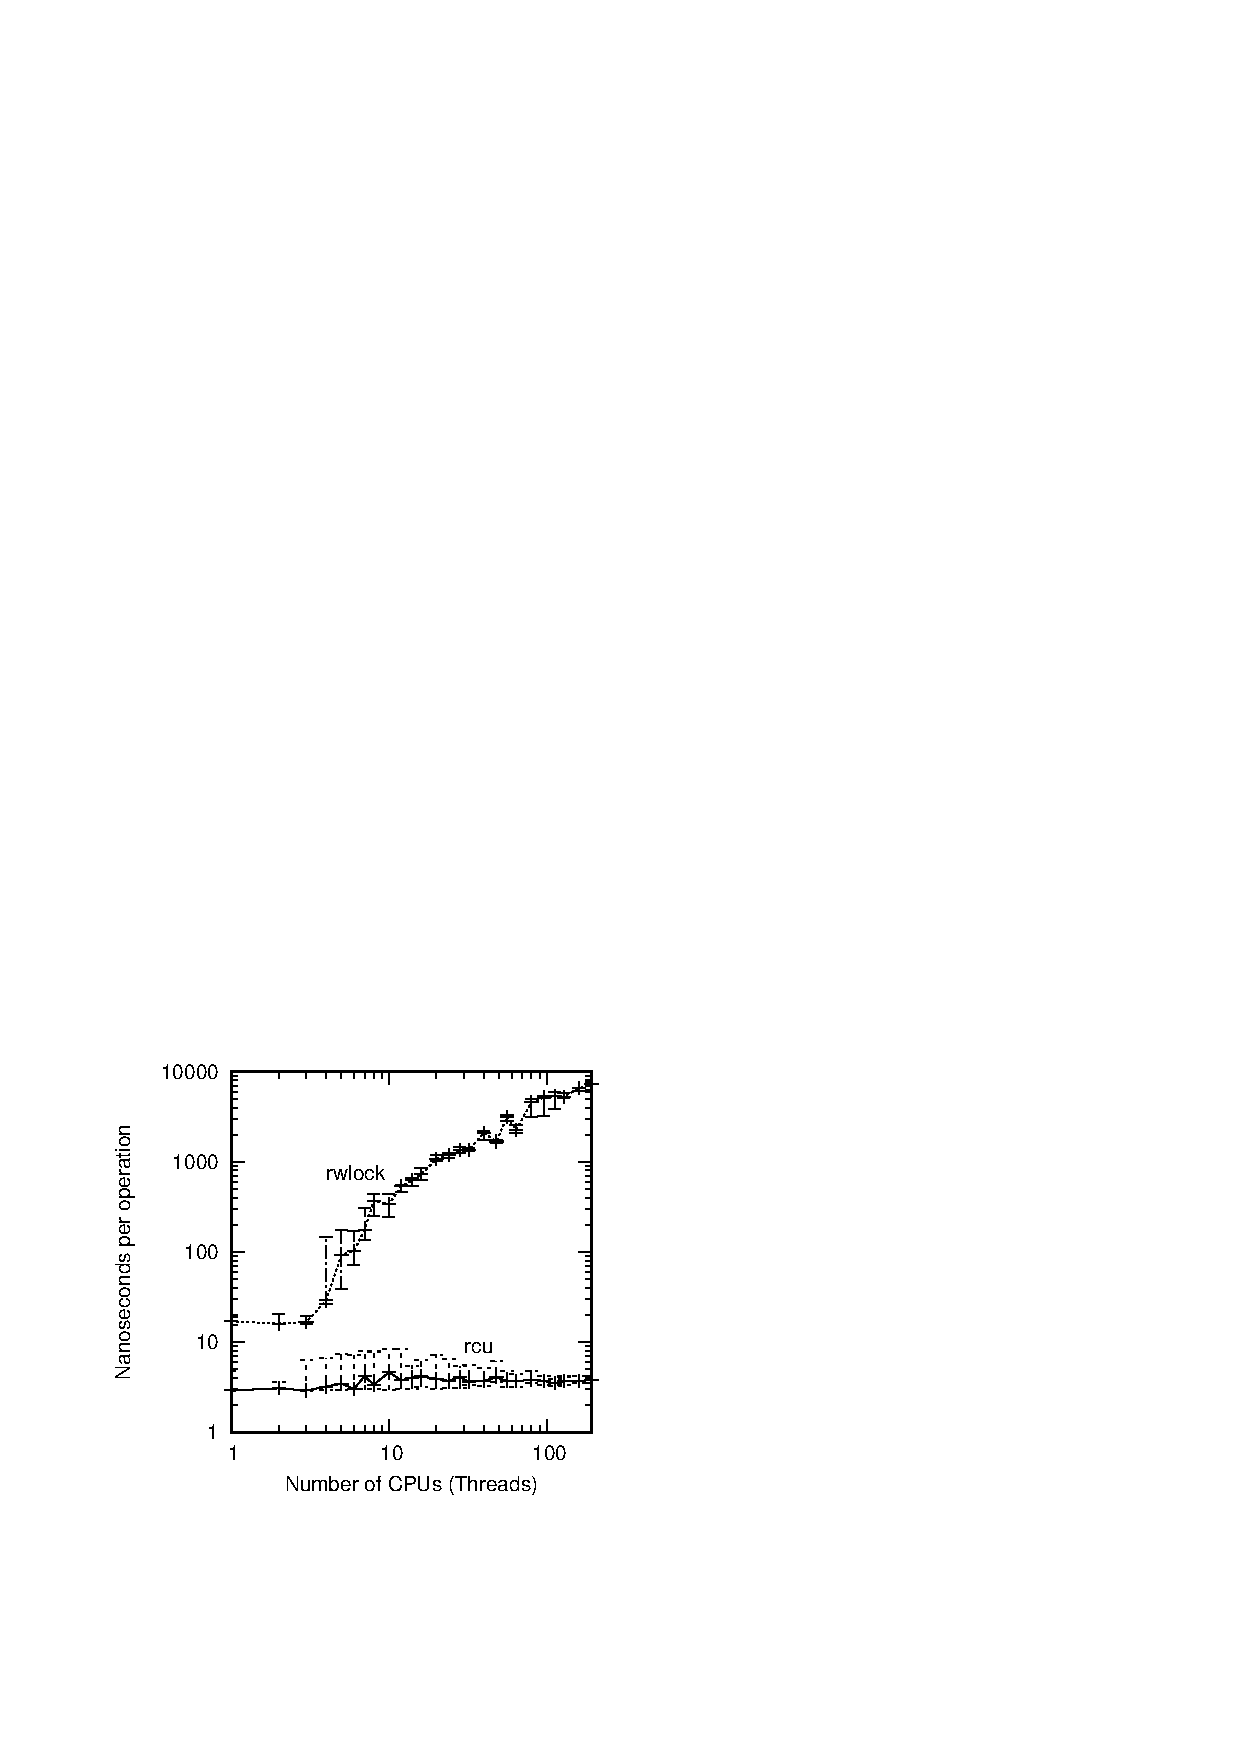
\includegraphics{defer/rwlockRCUperfPREEMPT}}
\end{center}
\caption{Performance Advantage of Preemptible RCU Over Reader-Writer Locking}
\label{fig:defer:Performance Advantage of Preemptible RCU Over Reader-Writer Locking}
\end{figure}

더 적당한 그림은 \co{CONFIG_PREEMPT} 커널에서 볼 수 있을텐데, 그렇다 하더라도
Figure~\ref{fig:defer:Performance Advantage of Preemptible RCU Over Reader-Writer Locking}
에서 볼 수 있듯이 RCU 는 여전히 reader-writer 락킹을 10배에서 1000배까지
압도하는 모습을 보입니다.
많은 수의 CPU 들에서의 reader-writer 락킹 성능의 높은 가변성을 보세요.
그림의 에러바들은 양쪽으로 표준편차만큼의 크기를 갖습니다.
\iffalse

A more moderate view may be obtained from a \co{CONFIG_PREEMPT}
kernel, though RCU still beats reader-writer locking by between one and
three orders of magnitude, as shown in
Figure~\ref{fig:defer:Performance Advantage of Preemptible RCU Over Reader-Writer Locking}.
Note the high variability of reader-writer locking at larger numbers of CPUs.
The error bars span a single standard deviation in either direction.
\fi

\begin{figure}[tb]
\begin{center}
\resizebox{3in}{!}{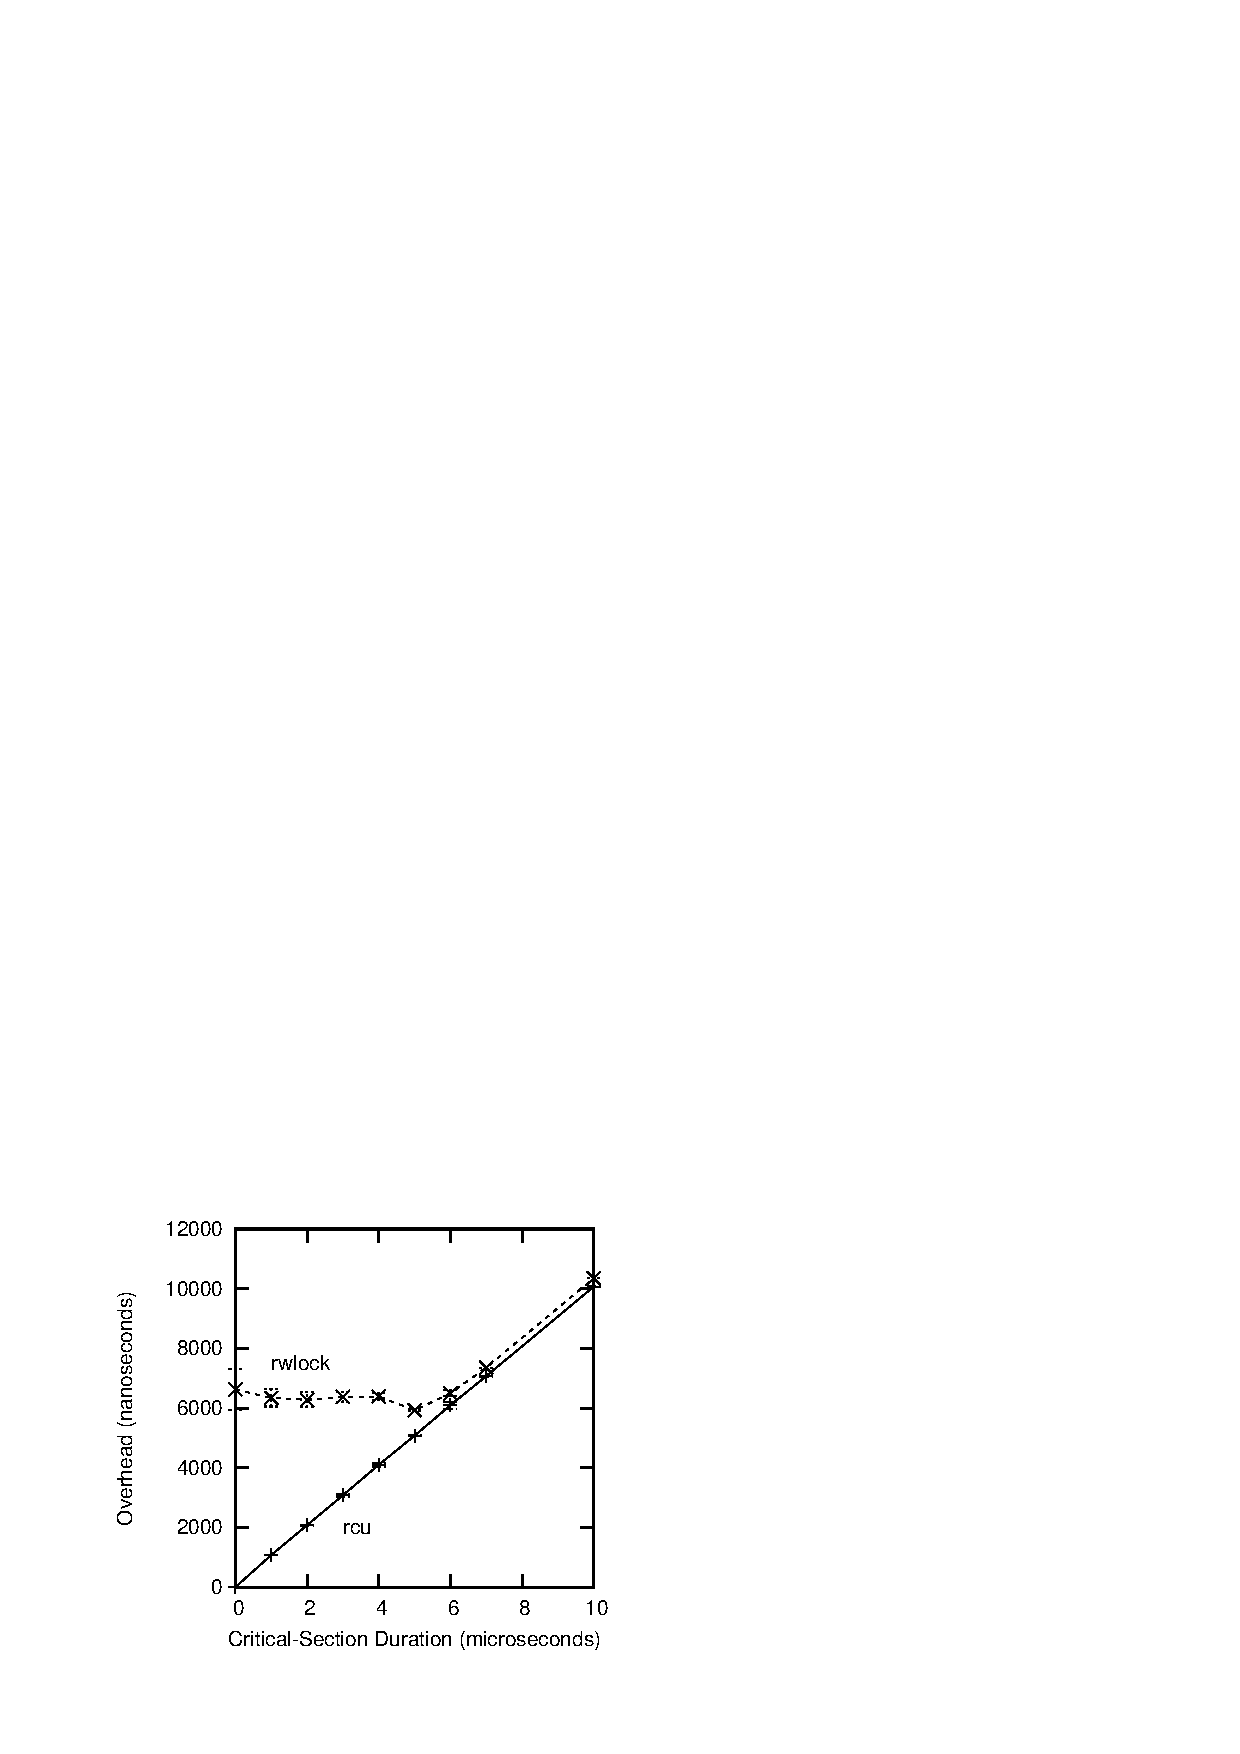
\includegraphics{defer/rwlockRCUperfwtPREEMPT}}
\end{center}
\caption{Comparison of RCU to Reader-Writer Locking as Function of Critical-Section Duration}
\label{fig:defer:Comparison of RCU to Reader-Writer Locking as Function of Critical-Section Duration}
\end{figure}

물론,
Figure~\ref{fig:defer:Performance Advantage of Preemptible RCU Over Reader-Writer Locking}
에 보인 reader-writer 락킹의 낮은 성능은 비현실적이게 짧은 크리티컬 섹션들로
인해 상당히 과장되었습니다.
RCU 의 성능상 이점은 16-CPU 환경에서 y 축은 read-side 기능들의 오버헤드와
크리티컬 섹션의 오버헤드의 합을 나타내는
Figure~\ref{fig:defer:Comparison of RCU to Reader-Writer Locking as Function of Critical-Section Duration}
에서 보인 것처럼, 크리티컬 섹션의 오버헤드가 늘어날수록 덜 뚜렷해집니다.
\iffalse

Of course, the low performance of reader-writer locking in
Figure~\ref{fig:defer:Performance Advantage of Preemptible RCU Over Reader-Writer Locking}
is exaggerated by the unrealistic zero-length critical sections.
The performance advantages of RCU become less significant as the overhead
of the critical section increases, as shown in
Figure~\ref{fig:defer:Comparison of RCU to Reader-Writer Locking as Function of Critical-Section Duration}
for a 16-CPU system,
in which the y-axis represents the sum of the overhead
of the read-side primitives and that of the critical section.
\fi

\QuickQuiz{}
	크리티컬 섹션 오버헤드가 늘어나면 왜 rwlock 의 오버헤드와 가변성이 모두
	줄어드는 거죠?
	\iffalse

	Why does both the variability and overhead of rwlock decrease as the
	critical-section overhead increases?
	\fi
\QuickQuizAnswer{
	크리티컬 섹션오버헤드가 증가하면 그 아래에 위치한 \co{rwlock_t} 를 얻기
	위한 경쟁이 줄어들기 때문입니다.
	하지만, 이 rwlock 오버헤드는 단일 CPU 에서는 캐시 쓰래싱 오버헤드
	때문에 그렇게 크게 떨어지지는 않을 겁니다.
	\iffalse

	Because the contention on the underlying
	\co{rwlock_t} decreases as the critical-section overhead
	increases.
	However, the rwlock overhead will not quite drop to that on a single
	CPU because of cache-thrashing overhead.
	\fi
} \QuickQuizEnd

하지만, 이 관측은 여러 시스템 콜들이 (그리고 따라서 그것들이 포함하고 있는 모든
RCU read-side 크리티컬 섹션들도) 수 마이크로세컨드 내에 완료될 수 있다는 사실에
맞춰서 좀 완화되어야만 합니다.

또한, 다음 섹션에서 이야기 되겠지만, RCU read-side 기능들은 거의 전부 데드락에
내성을 가지고 있습니다.
\iffalse

However, this observation must be tempered by the fact that
a number of system calls (and thus any RCU read-side critical sections
that they contain) can complete within a few microseconds.

In addition, as is discussed in the next section,
RCU read-side primitives are almost entirely deadlock-immune.
\fi


\paragraph{Deadlock Immunity}

RCU 가 읽기가 대부분인 워크로드에 상당한 성능 이득을 제공하긴 하지만, 사실 RCU
를 만들게 된 첫번째 목적은 read-side 의 데드락에 대한 내성입니다.
이 내성은 RCU 의 read-side 기능들은 블락도, 스피닝도, 심지어 뒤로 돌아가기도
하지 않으며, 따라서 그것들의 수행 시간이 결정론적이라는 사실에서 기인합니다.
따라서 이것들이 데드락 사이클에 연관되는 것은 불가능합니다.
\iffalse

Although RCU offers significant performance advantages for
read-mostly workloads, one of the primary reasons for creating
RCU in the first place was in fact its immunity to read-side
deadlocks.
This immunity stems from the fact that
RCU read-side primitives do not block, spin, or even
do backwards branches, so that their execution time is deterministic.
It is therefore impossible for them to participate in a deadlock
cycle.
\fi

\QuickQuiz{}
	이 데드락 내성에 어떤 예외가 있을까요, 그리고 만약 그렇다면, 어떤
	일련의 이벤트들이 데드락을 이끌어 낼 수 있을가요?
	\iffalse

	Is there an exception to this deadlock immunity, and if so,
	what sequence of events could lead to deadlock?
	\fi
\QuickQuizAnswer{
	RCU read-side 기능들이 연관된 데드락 사이클을 만들어내는 한가지 방법은
	다음과 같은 (불법적인) 일련의 코드들을 통해 가능합니다:
	\iffalse

	One way to cause a deadlock cycle involving
	RCU read-side primitives is via the following (illegal) sequence
	of statements:
	\fi

\vspace{5pt}
\begin{minipage}[t]{\columnwidth}
\small
\begin{verbatim}
rcu_read_lock();
synchronize_rcu();
rcu_read_unlock();
\end{verbatim}
\end{minipage}
\vspace{5pt}

	여기서의 \co{synchronize_srcu()} 는 전부터 존재한 모든 RCU read-side
	크리티컬 섹션이 완료되기 전까지 리턴할 수 없습니다만, 이 자체가 RCU
	read-side 크리티컬 섹션 안에 들어가 있고 그 크리티컬 섹션은
	\co{synchronize_rcu()} 가 리턴하기 전까지 끝날 수 없습니다.
	결국 이건 고전적인 self-deadlock 의 결과를 이끌어냅니다--읽기 모드로
	reader-writer 락을 잡은채로 쓰기 모드로 락을 잡으려 하면 똑같은 효과가
	나타날 겁니다.

	이 self-deadlock 시나리오는 RCU QSBR 에는 적용되지 않는다는 점을
	알아두셔야 하는데, 이는 \co{synchronize_rcu()} 에 의해 수행되는
	컨텍스트 스위치는 이 CPU 에 정지한 상태처럼 행동할 것이어서 grace
	period 가 완료되게 할 것이기 때문입니다.
	하지만, 이는 오히려 더 안좋은 케이스로, 이 RCU read-side 크리티컬
	섹션에 의해 사용되던 데이터가 해당 grace period 의 완료로 인해
	메모리에서 해제될 수 있기 때문입니다.

	짧게 말하자면, RCU read-side 크리티컬 섹션 내에서 동기적인 RCU
	update-side 기능들을 실행하지 마세요.
	\iffalse

	The \co{synchronize_rcu()} cannot return until all
	pre-existing RCU read-side critical sections complete, but
	is enclosed in an RCU read-side critical section that cannot
	complete until the \co{synchronize_rcu()} returns.
	The result is a classic self-deadlock---you get the same
	effect when attempting to write-acquire a reader-writer lock
	while read-holding it.

	Note that this self-deadlock scenario does not apply to
	RCU QSBR, because the context switch performed by the
	\co{synchronize_rcu()} would act as a quiescent state
	for this CPU, allowing a grace period to complete.
	However, this is if anything even worse, because data used
	by the RCU read-side critical section might be freed as a
	result of the grace period completing.

	In short, do not invoke synchronous RCU update-side primitives
	from within an RCU read-side critical section.
	\fi
} \QuickQuizEnd

RCU 의 read-side 데드락 내성의 흥미로운 결론은 무조건적으로 RCU 읽기 쓰레드를
RCU 업데이트 쓰레드로 업그레이드 시키는게 가능하다는 것입니다.
Reader-writer 락킹을 사용해서 그런 업그레이드를 하려 하면 데드락이 날 것입니다.
RCU read-to-update 업그레이드를 하는 예제 코드 조각은 다음과 같습니다:
\iffalse

An interesting consequence of RCU's read-side deadlock immunity is
that it is possible to unconditionally upgrade an RCU
reader to an RCU updater.
Attempting to do such an upgrade with reader-writer locking results
in deadlock.
A sample code fragment that does an RCU read-to-update upgrade follows:
\fi

\vspace{5pt}
\begin{minipage}[t]{\columnwidth}
\scriptsize
\begin{verbatim}
  1 rcu_read_lock();
  2 list_for_each_entry_rcu(p, &head, list_field) {
  3   do_something_with(p);
  4   if (need_update(p)) {
  5     spin_lock(my_lock);
  6     do_update(p);
  7     spin_unlock(&my_lock);
  8   }
  9 }
 10 rcu_read_unlock();
\end{verbatim}
\end{minipage}
\vspace{5pt}

\co{do_update()} 는 락의 보호 하에 실행되었다는 점, \emph{그리고} RCU read-side
보호 하에 실행되었다는 점에 주의하세요.

RCU 의 데드락 내성의 또다른 흥미로운 결론은 우선순위 역전 문제의 커다란
클래스에의 내성입니다.
예를 들어, 낮은 우선순위 RCU 읽기 쓰레드들은 높은 우선순위의 RCU 업데이트
쓰레드가 update-side 락을 잡는 걸 막을 수 없습니다.
유사하게, 낮은 우선순위 RCU 업데이트 쓰레드는 높은 우선순위 RCU 읽기 쓰레드들이
RCU read-side 크리티컬 섹션에 들어가는걸 막을 수 없습니다.
\iffalse

Note that \co{do_update()} is executed under
the protection of the lock \emph{and} under RCU read-side protection.

Another interesting consequence of RCU's deadlock immunity is its
immunity to a large class of priority inversion problems.
For example, low-priority RCU readers cannot prevent a high-priority
RCU updater from acquiring the update-side lock.
Similarly, a low-priority RCU updater cannot prevent high-priority
RCU readers from entering an RCU read-side critical section.
\fi

\QuickQuiz{}
	데드락과 우선순위 역전 모두에 내성이 있다고요???
	사실이라기엔 너무 좋은 이야기 같은데요.
	제가 이게 가능하다는걸 어떻게 믿을 수 있을까요?
	\iffalse

	Immunity to both deadlock and priority inversion???
	Sounds too good to be true.
	Why should I believe that this is even possible?
	\fi
\QuickQuizAnswer{
	정말로 잘 동작합니다.
	무엇보다, 이게 동작하지 않는다면, 리눅스 커널은 동작하지 못하겠죠.
	\iffalse

	It really does work.
	After all, if it didn't work, the Linux kernel would not run.
	\fi
} \QuickQuizEnd

\paragraph{Realtime Latency}

RCU read-side 기능들은 스피닝도 블락도 하지 않으므로, 훌륭한 리얼타임
대기시간을 제공합니다.
추가적으로, 앞에서도 이야기했듯, 이 말은 RCU read-side 기능들과 락들에 관련된
우선순위 역전 문제에도 내성이 있음을 뜻합니다.

하지만, RCU 는 좀 더 미묘한 우선순위 역전 시나리오에는 취약한데, 예를 들어, -rt
커널에서 어떤 RCU grace period 가 종료되기를 기다리느라 블락되어 있는 높은
우선순위의 프로세스는 낮은 우선순위의 RCU 읽기 쓰레드에 의해 블락될 수
있습니다.
이 문제는 RCU priority
boosting~\cite{PaulEMcKenney2007BoostRCU,DinakarGuniguntala2008IBMSysJ} 에 의해
해결될 수 있습니다.
\iffalse

Because RCU read-side primitives neither spin nor block, they offer
excellent realtime latencies.
In addition, as noted earlier, this means that they are
immune to priority inversion
involving the RCU read-side primitives and locks.

However, RCU is susceptible to more subtle priority-inversion scenarios,
for example, a high-priority process blocked waiting for an RCU
grace period to elapse can be blocked by low-priority RCU readers
in -rt kernels.
This can be solved by using RCU priority
boosting~\cite{PaulEMcKenney2007BoostRCU,DinakarGuniguntala2008IBMSysJ}.
\fi

\paragraph{RCU Readers and Updaters Run Concurrently}

RCU 읽기 쓰레드는 스핀도 블락도 하지 않고, 업데이트 쓰레드는 rollback 이나
abort 비슷한 것을 하지 않기 때문에, RCU 읽기 쓰레드와 업데이트 쓰레드는 동시에
수행될 수 있습니다.  이는 RCU 읽기 쓰레드는 낡은 데이터에 접근할 수 있고,
비일관적인 상태를 보게 될수 있어서, reader-writer 락킹에서 RCU 로의 변환이
간단하지 않을 것을 의미합니다.
\iffalse

Because RCU readers never spin nor block, and because updaters are not
subject to any sort of rollback or abort semantics, RCU readers and
updaters must necessarily run concurrently.
This means that RCU readers might access stale data, and might even
see inconsistencies, either of which can render conversion from reader-writer
locking to RCU non-trivial.
\fi

\begin{figure}[tb]
\begin{center}
\resizebox{3in}{!}{\includegraphics{defer/rwlockRCUupdate}}
\end{center}
\caption{Response Time of RCU vs. Reader-Writer Locking}
\label{fig:defer:Response Time of RCU vs. Reader-Writer Locking}
\end{figure}

하지만, 놀랍도록 많은 상황에서 비일관성과 낡은 데이터가 문제 되지 않습니다.
그런 고전적인 예는 네트워킹 라우팅 테이블입니다.
라우팅 업데이트는 시스템에 가해지는데 상당한 시간 (몇초에서 심지어 몇분까지도)
을 필요로 할 수 있기 때문에, 시스템은 업데이트가 도착했을 때 상당한 시간동안은
패킷들을 잘못된 방향으로 보낼 수도 있습니다.
몇 밀리세컨드동안 잘못된 방향으로 업데이트를 보내는 건 일반적으로 문제가 되지
않습니다.
더욱이, RCU 업데이트 쓰레드는 RCU 읽기 쓰레드가 끝나기를 기다리지 않고 변경을
가하기 때문에, RCU 읽기 쓰레드는 이 변경을 reader-writer 락킹의 읽기 쓰레드보다
빠르게 볼 수 있게 되는데,
Figure~\ref{fig:defer:Response Time of RCU vs. Reader-Writer Locking} 에 이
점이 그려져 있습니다.
\iffalse

However, in a surprisingly large number of situations, inconsistencies and
stale data are not problems.
The classic example is the networking routing table.
Because routing updates can take considerable time to reach a given
system (seconds or even minutes), the system will have been sending
packets the wrong way for quite some time when the update arrives.
It is usually not a problem to continue sending updates the wrong
way for a few additional milliseconds.
Furthermore, because RCU updaters can make changes without waiting for
RCU readers to finish,
the RCU readers might well see the change more quickly than would
batch-fair
reader-writer-locking readers, as shown in
Figure~\ref{fig:defer:Response Time of RCU vs. Reader-Writer Locking}.
\fi

일단 업데이트가 도착하면, rwlock 쓰기 쓰레드는 마지막 읽기 쓰레드가 완료되기
전까지, 뒤따르는 읽기 쓰레드는 이 쓰기가 완료되기 전까지 진행될 수 없습니다.
하지만, 뒤의 읽기 쓰레드는 새로운 값을 볼것이 보장되는데, 가장 오른쪽
박스들의 녹색 색깔로 표시되어 있습니다.
반면, RCU 읽기 쓰레드와 업데이트 쓰레드는 서로를 막지 않아, RCU 읽기 쓰레드가
업데이트된 값을 더 빨리 볼 수 있게 합니다.
물론, RCU 업데이트 쓰레드와 겹쳐 수행되기 때문에, 업데이트 전에 시작된 세개의
읽기 쓰레드를 포함해 \emph{모든} RCU 읽기 쓰레드는 업데이트된 값을 보게 될수도
있을겁니다.
하지만 가장 오른쪽의 녹색으로 칠해진 RCU 읽기 쓰레드들만이 업데이트된 값을 볼
것이 \emph{보장됩니다}.
\iffalse

Once the update is received, the rwlock writer cannot proceed until the
last reader completes, and subsequent readers cannot proceed until the
writer completes.
However, these subsequent readers are guaranteed to see the new value,
as indicated by the green shading of the rightmost boxes.
In contrast, RCU readers and updaters do not block each other, which permits
the RCU readers to see the updated values sooner.
Of course, because their execution overlaps that of the RCU updater,
\emph{all} of the RCU readers might well see updated values, including
the three readers that started before the update.
Nevertheless only the green-shaded rightmost RCU readers
are \emph{guaranteed} to see the updated values.
\fi

Reader-writer 락킹과 RCU 는 그저 다른 보장을 제공합니다.
Reader-writer 락킹에서는, 쓰기 쓰레드보다 시작을 늦게 한 읽기 쓰레드는 모두 새
값을 볼 것이 보장되고, 쓰기 쓰레드가 스피닝 하는중에 시작되려 시도하는 읽기
쓰레드는 rwlock 의 읽기/쓰기 우선권 구현에 따라 새 값을 볼수도 못볼수도
있습니다.
반면에, RCU 에서는 업데이트 쓰레드가 완료된 후에 시작된 읽기 쓰레드는 모두 새
값을 볼것이 보장되고, 업데이트가 시작된 후에 완료된 모든 읽기 쓰레드는 타이밍에
따라 새 값을 볼수도 못볼수도 있습니다.
\iffalse

Reader-writer locking and RCU simply provide different guarantees.
With reader-writer locking, any reader that begins after the writer begins
is guaranteed to see new values, and any reader that attempts to
begin while the writer is spinning might or might not see new values,
depending on the reader/writer preference of the rwlock implementation in
question.
In contrast, with RCU, any reader that begins after the updater completes
is guaranteed to see new values, and any reader that completes after the
updater begins might or might not see new values, depending on timing.
\fi

여기서의 핵심은, reader-writer 락킹이 컴퓨터 시스템에 국한해서는 실제로
일관성을 보장하지만, 이 일관성이 그 바깥 세계에서는 더 증가된 \emph{비일관성}
이라는 비용이 되는 상황이 존재한다는 것입니다.
달리 말해, reader-writer 락킹은 바깥 세계의 관점에서는 조용히 망가져버린
데이터의 비용으로 내부의 일관성을 얻습니다.
\iffalse

The key point here is that, although reader-writer locking does
indeed guarantee consistency within the confines of the computer system,
there are situations where this consistency comes at the price of
increased \emph{inconsistency} with the outside world.
In other words, reader-writer locking obtains internal consistency at the
price of silently stale data with respect to the outside world.
\fi

그러나, 시스템에 국한된 비일관성과 망가진 데이터가 허용될 수 없는 상황이
존재합니다.
다행히도, 비일관성과 망가진 데이터를 방지하는 방법들이
여럿~\cite{PaulEdwardMcKenneyPhD,Arcangeli03} 있고, 일부 방법은
Section~\ref{sec:defer:Reference Counting} 에서 논의한 레퍼런스 카운팅에
기반합니다.
\iffalse

Nevertheless, there are situations where inconsistency and stale
data within the confines of the system cannot be tolerated.
Fortunately,
there are a number of approaches that avoid inconsistency and stale
data~\cite{PaulEdwardMcKenneyPhD,Arcangeli03}, and some
methods based on reference counting are discussed in
Section~\ref{sec:defer:Reference Counting}.
\fi

\paragraph{Low-Priority RCU Readers Can Block High-Priority Reclaimers}

리얼타임 RCU~\cite{DinakarGuniguntala2008IBMSysJ},
SRCU~\cite{PaulEMcKenney2006c}, 또는
QRCU~\cite{PaulEMcKenney2007QRCUspin} (
Section~\ref{sec:formal:Promela Example: QRCU} 를 참고하세요) 에서,
preemption 당한 읽기 쓰레드는 grace period 가 종료되는 걸 막을 것인데, 높은
우선순위 태스크가 해당 grace period 가 완료되기를 기다리느라 블락되어 있더라도
그럴 겁니다.
리얼타임 RCU 는 \co{call_rcu()} 를 \co{synchronize_rcu()} 로 대체하거나 2008년
초인 지금 시점까지는 아직 실험적 단계인 RCU priority
boosting~\cite{PaulEMcKenney2007BoostRCU,DinakarGuniguntala2008IBMSysJ} 을
사용해서 이 문제를 해결 할 수 있습니다.
SRCU 와 QRCU 에 priority boosting 을 합치는게 필요할 수도 있겠지만, 그전에
실제 세계에서의 분명한 필요성이 보여져야 합니다.
\iffalse

In Realtime RCU~\cite{DinakarGuniguntala2008IBMSysJ},
SRCU~\cite{PaulEMcKenney2006c}, or
QRCU~\cite{PaulEMcKenney2007QRCUspin} (see
Section~\ref{sec:formal:Promela Example: QRCU}),
a preempted reader will prevent
a grace period from completing, even if a high-priority task is
blocked waiting for that grace period to complete.
Realtime RCU can avoid this problem by substituting \co{call_rcu()}
for \co{synchronize_rcu()} or by using RCU priority
boosting~\cite{PaulEMcKenney2007BoostRCU,DinakarGuniguntala2008IBMSysJ},
which is still in experimental status as of early 2008.
It might become necessary to augment SRCU and QRCU with priority boosting,
but not before a clear real-world need is demonstrated.
\fi

\paragraph{RCU Grace Periods Extend for Many Milliseconds}

QRCU 와
Appendix~\ref{chp:app:``Toy'' RCU Implementations} 에 설명된 몇개의 ``장난감''
RCU 구현들의 예외가 있지만, RCU grace period 들은 여러 밀리세컨드까지
늘어납니다.
사용 가능한 비동기적인 인터페이스 (\co{call_rcu()} 와 \co{call_rcu_bh()}) 를
사용하는 방법을 포함해, 그런 긴 딜레이를 위험하지 않게 만드는 몇가지 테크닉들이
있긴 하지만, 이 상황은 RCU 가 읽기가 대부분인 상황에서만 사용되어야 한다는
규칙의 주요 이유입니다.
\iffalse

With the exception of QRCU and several of the ``toy'' RCU implementations
described in
Appendix~\ref{chp:app:``Toy'' RCU Implementations},
RCU grace periods extend for multiple milliseconds.
Although there are a number of techniques to render such long delays
harmless, including use of the asynchronous interfaces where available
(\co{call_rcu()} and \co{call_rcu_bh()}), this situation
is a major reason for the rule of thumb that RCU be used in read-mostly
situations.
\fi

\paragraph{Comparison of Reader-Writer Locking and RCU Code}

적합한 경우에 reader-writer 락킹에서 RCU 로의 변경은
위키피디아에서 가져온~\cite{WikipediaRCU}
Figure~\ref{lst:defer:Converting Reader-Writer Locking to RCU: Data},
\ref{lst:defer:Converting Reader-Writer Locking to RCU: Search},
그리고
\ref{lst:defer:Converting Reader-Writer Locking to RCU: Deletion}
에서처럼 매우 간단합니다.
\iffalse


In the best case, the conversion from reader-writer locking to RCU
is quite simple, as shown in
Listings~\ref{lst:defer:Converting Reader-Writer Locking to RCU: Data},
\ref{lst:defer:Converting Reader-Writer Locking to RCU: Search},
and
\ref{lst:defer:Converting Reader-Writer Locking to RCU: Deletion},
all taken from
Wikipedia~\cite{WikipediaRCU}.
\fi

\begin{listing*}[htbp]
{ \scriptsize
\begin{verbbox}
 1 struct el {                           1 struct el {
 2   struct list_head lp;                2   struct list_head lp;
 3   long key;                           3   long key;
 4   spinlock_t mutex;                   4   spinlock_t mutex;
 5   int data;                           5   int data;
 6   /* Other data fields */             6   /* Other data fields */
 7 };                                    7 };
 8 DEFINE_RWLOCK(listmutex);             8 DEFINE_SPINLOCK(listmutex);
 9 LIST_HEAD(head);                      9 LIST_HEAD(head);
\end{verbbox}
}
\hspace*{0.9in}\OneColumnHSpace{-0.5in}
\theverbbox
\caption{Converting Reader-Writer Locking to RCU: Data}
\label{lst:defer:Converting Reader-Writer Locking to RCU: Data}
\end{listing*}

\begin{listing*}[htbp]
{ \scriptsize
\begin{verbbox}
 1 int search(long key, int *result)     1 int search(long key, int *result)
 2 {                                     2 {
 3   struct el *p;                       3   struct el *p;
 4                                       4
 5   read_lock(&listmutex);              5   rcu_read_lock();
 6   list_for_each_entry(p, &head, lp) { 6   list_for_each_entry_rcu(p, &head, lp) {
 7     if (p->key == key) {              7     if (p->key == key) {
 8       *result = p->data;              8       *result = p->data;
 9       read_unlock(&listmutex);        9       rcu_read_unlock();
10       return 1;                      10       return 1;
11     }                                11     }
12   }                                  12   }
13   read_unlock(&listmutex);           13   rcu_read_unlock();
14   return 0;                          14   return 0;
15 }                                    15 }
\end{verbbox}
}
\hspace*{0.9in}\OneColumnHSpace{-0.5in}
\theverbbox
\caption{Converting Reader-Writer Locking to RCU: Search}
\label{lst:defer:Converting Reader-Writer Locking to RCU: Search}
\end{listing*}

\begin{listing*}[htbp]
{ \scriptsize
\begin{verbbox}
 1 int delete(long key)                  1 int delete(long key)
 2 {                                     2 {
 3   struct el *p;                       3   struct el *p;
 4                                       4
 5   write_lock(&listmutex);             5   spin_lock(&listmutex);
 6   list_for_each_entry(p, &head, lp) { 6   list_for_each_entry(p, &head, lp) {
 7     if (p->key == key) {              7     if (p->key == key) {
 8       list_del(&p->lp);               8       list_del_rcu(&p->lp);
 9       write_unlock(&listmutex);       9       spin_unlock(&listmutex);
                                        10       synchronize_rcu();
10       kfree(p);                      11       kfree(p);
11       return 1;                      12       return 1;
12     }                                13     }
13   }                                  14   }
14   write_unlock(&listmutex);          15   spin_unlock(&listmutex);
15   return 0;                          16   return 0;
16 }                                    17 }
\end{verbbox}
}
\hspace*{0.9in}\OneColumnHSpace{-0.5in}
\theverbbox
\caption{Converting Reader-Writer Locking to RCU: Deletion}
\label{lst:defer:Converting Reader-Writer Locking to RCU: Deletion}
\end{listing*}

Reader-writer 락킹을 RCU 로 바꾸는 더 정교한 경우들은 이 문서의 범위 밖입니다.
\iffalse

More-elaborate cases of replacing reader-writer locking with RCU
are beyond the scope of this document.
\fi

\subsubsection{RCU is a Restricted Reference-Counting Mechanism}
\label{sec:defer:RCU is a Restricted Reference-Counting Mechanism}

RCU read-side 크리티컬 섹션이 진행중인 동안은 grace period 들이 완료될 수 없기
때문에, RCU read-side 기능들은 제한적인 레퍼런스 카운팅 메커니즘으로 사용될수도
있습니다.
예를 들어, 다음과 같은 코드 조각을 생각해 봅시다:
\iffalse

Because grace periods are not allowed to complete while
there is an RCU read-side critical section in progress,
the RCU read-side primitives may be used as a restricted
reference-counting mechanism.
For example, consider the following code fragment:
\fi

\vspace{5pt}
\begin{minipage}[t]{\columnwidth}
\scriptsize
\begin{verbatim}
  1 rcu_read_lock();  /* acquire reference. */
  2 p = rcu_dereference(head);
  3 /* do something with p. */
  4 rcu_read_unlock();  /* release reference. */
\end{verbatim}
\end{minipage}
\vspace{5pt}

이 \co{rcu_read_lock()} 는 \co{p} 로의 레퍼런스를 얻어오는 것으로 볼 수
있는데, \co{rcu_dereference()} 를 통한 \co{p} 로의 할당 후 시작되는 grace
period 는 연관되는 \co{rcu_read_unlock()} 전까지는 끝나지 않을
것이기 때문입니다.
이 레퍼런스 카운팅 방식은 RCU read-side 크리티컬 섹션 안에서는
블락이 허용되지 않고, 다른 태스크로 RCU read-side 크리티컬
섹션을 넘겨줄 수도 없다는 점에서 제한적입니다.

그런 제한에도 불구하고, 다음의 코드는 안전하게 \co{p} 를 삭제할 수 있습니다:
\iffalse

The \co{rcu_read_lock()} primitive can be thought of as
acquiring a reference to \co{p}, because a grace period
starting after the \co{rcu_dereference()} assigns to \co{p}
cannot possibly end until after we reach the matching
\co{rcu_read_unlock()}.
This reference-counting scheme is restricted in that
we are not allowed to block in RCU read-side critical sections,
nor are we permitted to hand off an RCU read-side critical section
from one task to another.

Regardless of these restrictions,
the following code can safely delete \co{p}:
\fi

\vspace{5pt}
\begin{minipage}[t]{\columnwidth}
\scriptsize
\begin{verbatim}
  1 spin_lock(&mylock);
  2 p = head;
  3 rcu_assign_pointer(head, NULL);
  4 spin_unlock(&mylock);
  5 /* Wait for all references to be released. */
  6 synchronize_rcu();
  7 kfree(p);
\end{verbatim}
\end{minipage}
\vspace{5pt}

\co{head} 로의 할당은 뒤이은 \co{p} 로의 레퍼런스 획득을 방지하고,
\co{synchronize_rcu()} 는 앞서 획득된 레퍼런스들이 해제되기를 기다립니다.
\iffalse

The assignment to \co{head} prevents any future references
to \co{p} from being acquired, and the \co{synchronize_rcu()}
waits for any previously acquired references to be released.
\fi

\QuickQuiz{}
	근데 잠깐만요!
	이건 RCU 를 reader-writer 락킹 대용으로 하려 할 때 쓸법한 코드와 완전
	똑같잖아요!
	뭐가 새로운 거죠?
	\iffalse

	But wait!
	This is exactly the same code that might be used when thinking
	of RCU as a replacement for reader-writer locking!
	What gives?
	\fi
\QuickQuizAnswer{
	이는 장난감 예제의 법칙의 효과입니다:
	어떤 특정 포인트 이후로는 해당 코드는 똑같아 보일 겁니다.
	이 코드를 어떻게 생각하느냐가 단 하나의 차이입니다.
	하지만, 이 차이점은 매우 중요할 수 있습니다.
	이 중요성에 대해 한가지만 예를 들어, RCU 를 레퍼런스 카운팅 방법으로
	생각하고 있다고 치면, 업데이트들이 RCU read-side 크리티컬 섹션들을
	배제할거라 생각하는 실수를 하지 않을 겁니다.

	더도 아니고 덜도 아니고 RCU 를 reader-writer 락킹의 대체제로 생각하는
	건 종종 쓸모있는데, 예를 들면 reader-writer 락킹을 RCU 로 대체할
	때입니다.
	\iffalse

	This is an effect of the Law of Toy Examples:
	beyond a certain point, the code fragments look the same.
	The only difference is in how we think about the code.
	However, this difference can be extremely important.
	For but one example of the importance, consider that if we think
	of RCU as a restricted reference counting scheme, we would never
	be fooled into thinking that the updates would exclude the RCU
	read-side critical sections.

	It nevertheless is often useful to think of RCU as a replacement
	for reader-writer locking, for example, when you are replacing
	reader-writer locking with RCU.
	\fi
} \QuickQuizEnd

물론, RCU 는 Section~\ref{sec:together:Refurbish Reference Counting} 에서
논의된 것처럼, 전통적인 레퍼런스 카운팅과 함께 조합될 수도 있습니다.
\iffalse

Of course, RCU can also be combined with traditional reference counting,
as discussed in
Section~\ref{sec:together:Refurbish Reference Counting}.
\fi

\begin{figure}[tb]
\begin{center}
\resizebox{3in}{!}{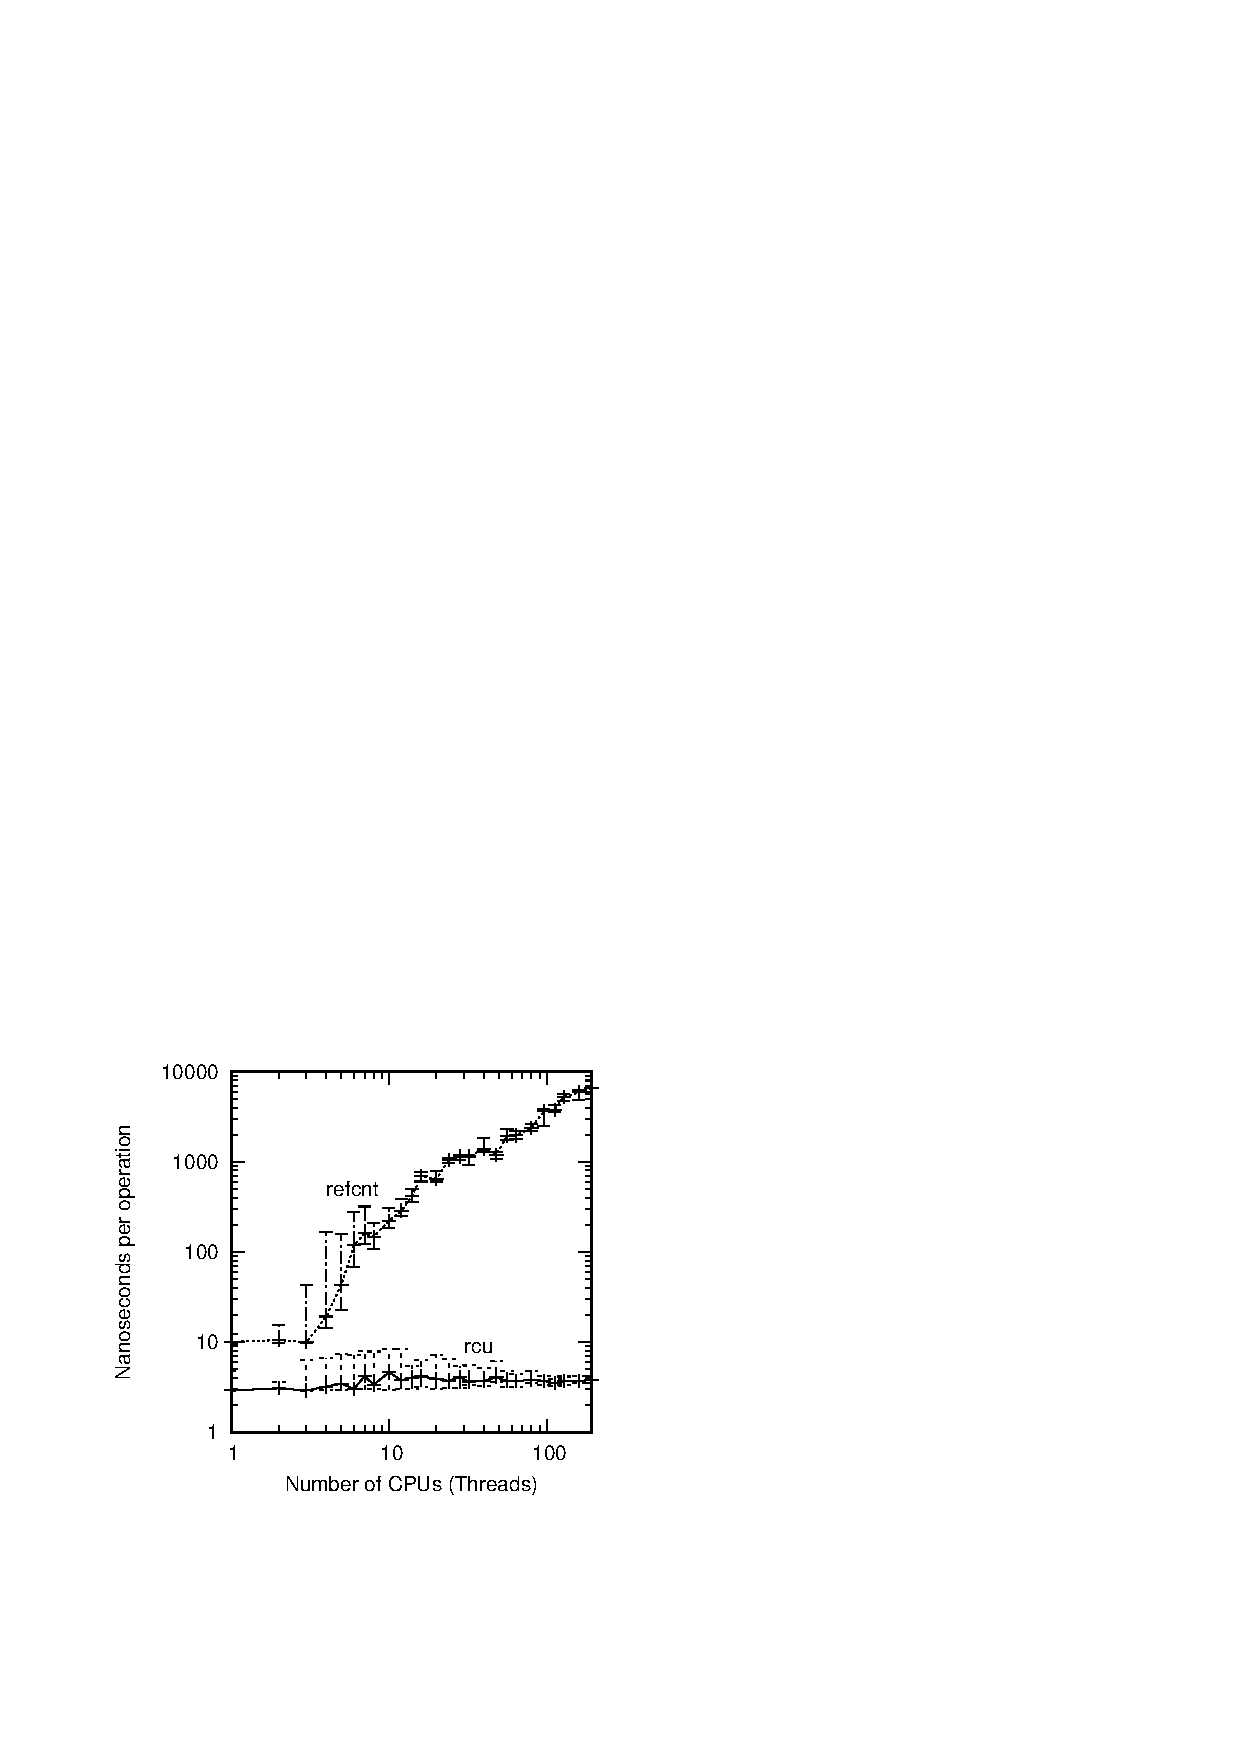
\includegraphics{defer/refRCUperfPREEMPT}}
\end{center}
\caption{Performance of RCU vs. Reference Counting}
\label{fig:defer:Performance of RCU vs. Reference Counting}
\end{figure}

하지만 왜 이런 신경을 쓰는 걸까요?
다시 말하지만, 답 중 하나는 성능으로, 16-CPU 3GHz Intel x86 시스템에서의
데이터가
Figure~\ref{fig:defer:Performance of RCU vs. Reference Counting} 에 있습니다.
\iffalse

But why bother?
Again, part of the answer is performance, as shown in
Figure~\ref{fig:defer:Performance of RCU vs. Reference Counting},
again showing data taken on a 16-CPU 3\,GHz Intel x86 system.
\fi

\QuickQuiz{}
	6 CPU 근처에서 refcnt 오버헤드가 확 떨어지는건 왜그렇죠?
	\iffalse

	Why the dip in refcnt overhead near 6 CPUs?
	\fi
\QuickQuizAnswer{
	NUMA 효과 때문일 겁니다.
	하지만, 에러 바들로 보여진 것처럼, refcnt 선을 측정하는데 사용된 값들은
	상당한 편차를 가지고 있습니다.
	사실, 일부 케이스에 있어서 표준편차는 측정된 값의 10\,\% 를 초과합니다.
	따라서 해당 오버헤드의 큰 차이는 통계적 탈선일 수도 있습니다.
	\iffalse

	Most likely NUMA effects.
	However, there is substantial variance in the values measured for the
	refcnt line, as can be seen by the error bars.
	In fact, standard deviations range in excess of 10\,\% of measured
	values in some cases.
	The dip in overhead therefore might well be a statistical aberration.
	\fi
} \QuickQuizEnd

\begin{figure}[tb]
\begin{center}
\resizebox{3in}{!}{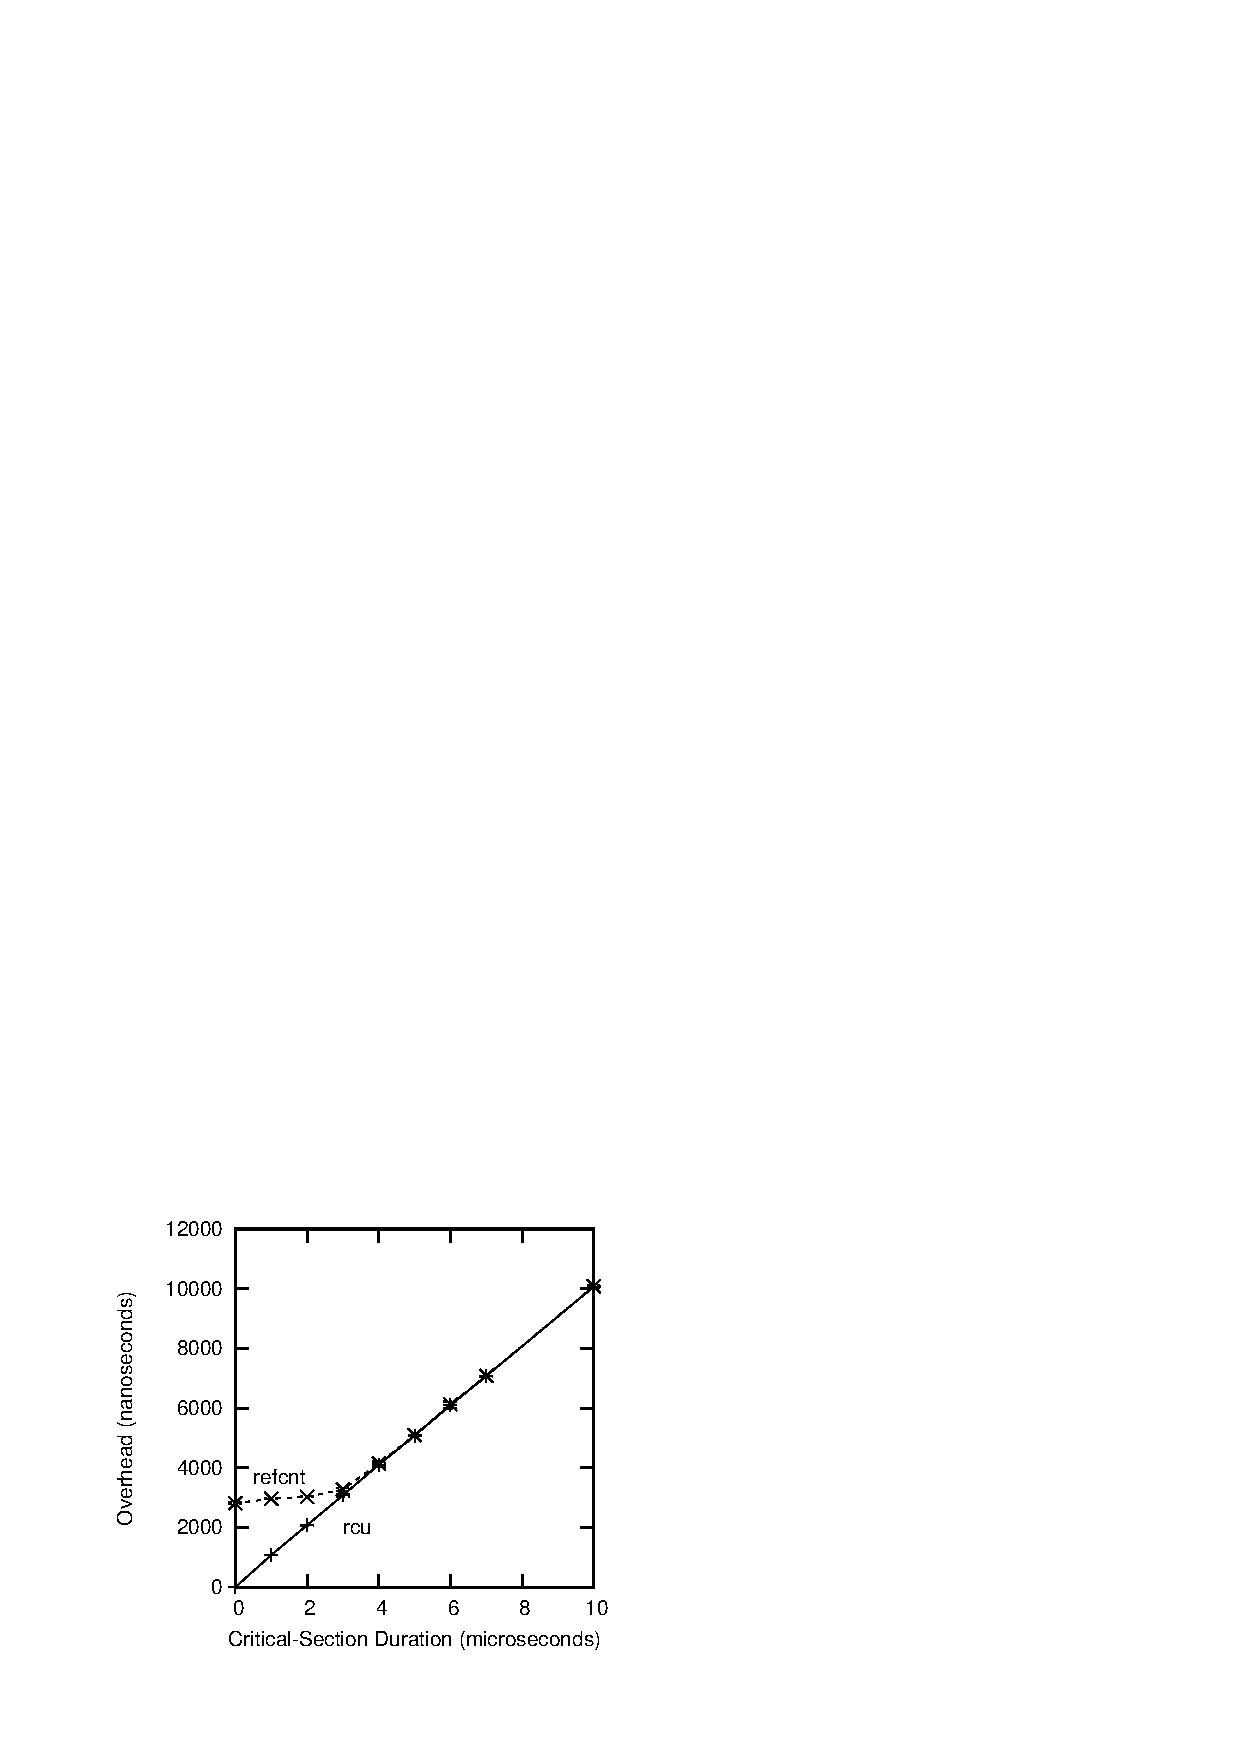
\includegraphics{defer/refRCUperfwtPREEMPT}}
\end{center}
\caption{Response Time of RCU vs. Reference Counting}
\label{fig:defer:Response Time of RCU vs. Reference Counting}
\end{figure}

그리고, reader-writer 락킹 때처럼, RCU 의 성능상 이득은
Figure~\ref{fig:defer:Response Time of RCU vs. Reference Counting} 에 16-CPU
시스템에서의 결과로 보여지듯 짧은 길이의 크리티컬 섹션들에서 가장 효과를
발합니다.
또한, reader-writer 락킹에서처럼, 많은 시스템 콜들은 (그리고 그것들을 포함하는
RCU read-side 크리티컬 섹션들은) 수 마이크로세컨드 내에 끝납니다.
\iffalse

And, as with reader-writer locking, the performance advantages
of RCU are most pronounced for short-duration critical sections, as shown
Figure~\ref{fig:defer:Response Time of RCU vs. Reference Counting}
for a 16-CPU system.
In addition, as with reader-writer locking, many system calls (and thus
any RCU read-side critical sections that they contain) complete in
a few microseconds.
\fi

하지만, RCU 에 따라오는 이 제약들은 상당히 성가십니다.
예를 들어, 많은 경우에 RCU read-side 크리티컬 섹션 내에서 잠들기가 금지된다는
점은 목표 달성을 불가하게 할 수 있습니다.
다음 섹션에서는 적어도 일부 경우에서는 전통적 레퍼런스 카운팅의 복잡도를
낮추면서도 이 문제를 해결하는 방법들을 알아보겠습니다.
\iffalse

However, the restrictions that go with RCU can be quite onerous.
For example, in many cases, the prohibition against sleeping while in an RCU
read-side critical section would defeat the entire purpose.
The next section looks at ways of addressing this problem, while also
reducing the complexity of traditional reference counting, at least in
some cases.
\fi

\subsubsection{RCU is a Bulk Reference-Counting Mechanism}
\label{sec:defer:RCU is a Bulk Reference-Counting Mechanism}

앞의 섹션에서 이야기 했듯, 전통적인 레퍼런스 카운터들은 보통 특정 데이터 구조
또는 데이터 구조체들의 특정 그룹과 연관되어 있습니다.
하지만, 매우 다양한 데이터 구조체들에 하나의 글로벌한 레퍼런스 카운터를
사용하는 것은 이 레퍼런스 카운트를 담고 있는 캐시 라인 바운싱 (cache line
bouncing) 을 초래합니다.
그런 캐시 라인 바운싱은 성능을 심각하게 저하시킬 수 있습니다.
\iffalse

As noted in the preceding section,
traditional reference counters are usually associated with a specific
data structure, or perhaps a specific group of data structures.
However, maintaining a single global reference counter for a large
variety of data structures typically results in bouncing
the cache line containing the reference count.
Such cache-line bouncing can severely degrade performance.
\fi

반면, RCU 의 가벼운 read-side 기능들은 무시해도 좋을 만한 성능 저하만을
가지면서 굉장히 빈번한 read-side 실행이 가능하게 해서 적거나 아예 없는 퍼포먼스
저하를 갖는 ``벌크 레퍼런스 카운팅'' 메커니즘으로 RCU 가 사용될 수 있습니다.
블록을 하는 코드 섹션들을 가로질러 하나의 태스크가 하나의 레퍼런스를 쥐고
있어야만 하는 상황에는 Sleepable RCU (SRCU)~\cite{PaulEMcKenney2006c} 가 사용될
수 있을 겁니다.
이는 레퍼런스가 한 태스크에서 다른 태스크로 ``전달'' 되는, 예를 들어 레퍼런스가
I/O 의 시작에 획득되어지고 연관된 완료 인터럽트 핸들러에서 해제되는, 희귀하지
않은 상황들을 처리하지는 못할 겁니다.
(원칙적으로, 이는 SRCU 구현으로 처리될 수도 있지만, 실제로 이게 좋은
트레이드오프인지가는 아직 명확하지 않습니다.)
\iffalse

In contrast, RCU's light-weight read-side primitives permit
extremely frequent read-side usage with negligible performance
degradation, permitting RCU to be used as a ``bulk reference-counting''
mechanism with little or no performance penalty.
Situations where a reference must be held by a single task across a
section of code that blocks may be accommodated with
Sleepable RCU (SRCU)~\cite{PaulEMcKenney2006c}.
This fails to cover the not-uncommon situation where a reference is ``passed''
from one task to another, for example, when a reference is acquired
when starting an I/O and released in the corresponding completion
interrupt handler.
(In principle, this could be handled by the SRCU implementation,
but in practice, it is not yet clear whether this is a good tradeoff.)
\fi

물론, SRCU 는 그 자신의 제약을 가지는데, \co{srcu_read_lock()} 의 리턴값은
연관된 \co{srcu_read_unlock()} 으로 전달되고, 어떤 SRCU 기능도 하드웨어
인터럽트 핸들러나 non-maskable interrupt (NMI) 핸들러 안에서 실행될 수 없다는
것입니다.
이런 제약들에 의해 얼마나 많은 문제들이 존재하게 되는지, 그리고 그것들이 어떻게
가장 잘 처리될 수 있는지에 대한 판단은 아직 진행 중입니다.
\iffalse

Of course, SRCU brings restrictions of its own, namely that the
return value from \co{srcu_read_lock()} be passed into the
corresponding \co{srcu_read_unlock()}, and that no SRCU primitives
be invoked from hardware interrupt handlers or from non-maskable interrupt
(NMI) handlers.
The jury is still out as to how much of a problem is presented by
these restrictions, and as to how they can best be handled.
\fi

\subsubsection{RCU is a Poor Man's Garbage Collector}
\label{sec:defer:RCU is a Poor Man's Garbage Collector}

RCU 를 처음 공부하는 사람들이 갖는, 희귀하지 않은 감탄 하나는 ``RCU 는 가비지
콜렉터 같은 것이다!'' 입니다.
이 감탄은 커다란 진실을 품고 있기는 하지만, 또한 오해가 될 수도 있습니다.
\iffalse

A not-uncommon exclamation made by people first learning about
RCU is ``RCU is sort of like a garbage collector!''
This exclamation has a large grain of truth, but it can also be
misleading.
\fi

RCU 와 자동화된 가비지 콜렉터들 (GC) 사이의 관계를 생각하는 가장 좋은 방법은
RCU 는 콜렉션의 \emph{타이밍} 이 자동으로 정해진다는 점에서 RCU 가 GC 와
닮았다는 점입니다만, RCU 는 GC 와 다음과 같이 다릅니다: (1) 프로그래머는 언제
특정 데이터 구조체가 정리되어도 좋은지를 일일이 알려야만 하고, (2) 프로그래머는
레퍼런스들이 합법적으로 붙잡힐 수 있는 RCU read-side 크리티컬 섹션들을 일일이
표시해야만 합니다.
\iffalse

Perhaps the best way to think of the relationship between RCU
and automatic garbage collectors (GCs) is that RCU resembles
a GC in that the \emph{timing} of collection is automatically
determined, but that RCU differs from a GC in that: (1) the programmer
must manually indicate when a given data structure is eligible
to be collected, and (2) the programmer must manually mark the
RCU read-side critical sections where references might legitimately
be held.
\fi

이런 차이점들에도 불구하고, 유사한 부분들 역시 상당히 깊은 영역까지 들어가는
편이고, RCU 에 대한 최소한 하나의 이론적인 분석이 될수도 있습니다.
더 나아가서, 제가 신경썼던 첫번째 RCU 같은 메커니즘은 grace period 를 처리하기
위해 가비지 콜렉터를 사용했습니다.
하지만 더도 아니고 덜도 아니고, RCU 를 생각하는 더 나은 방법은 다음 섹션에
설명되어 있습니다.
\iffalse

Despite these differences, the resemblance does go quite deep,
and has appeared in at least one theoretical analysis of RCU.
Furthermore, the first RCU-like mechanism I am aware of used
a garbage collector to handle the grace periods.
Nevertheless, a better way of thinking of RCU is described in the
following section.
\fi

\subsubsection{RCU is a Way of Providing Existence Guarantees}
\label{sec:defer:RCU is a Way of Providing Existence Guarantees}

Gamsa 등~\cite{Gamsa99} 은 존재 보장에 대해 논하고 어떻게 RCU 를 닮은
메커니즘이 이런 존재 보장을 제공하기 위해 사용되는지 설명 (해당 PDF 의 7
페이지의 section~5 를 보세요) 했고,
Section~\ref{sec:locking:Lock-Based Existence Guarantees} 에서는 존재 보장을
락킹을 사용해서 어떻게 하는지를 그렇게 하는 것의 단점과 함께 이야기했습니다.
만약 RCU 로 보호되는 데이터 원소가 RCU read-side 크리티컬 섹션 내에서
접근된다면, 그 데이터 항목은 그 RCU read-side 크리티컬섹션 기간 동안은 존재하는
상태로 유지되는 것이 보장됩니다.
\iffalse

Gamsa et al.~\cite{Gamsa99}
discuss existence guarantees and describe how a mechanism
resembling RCU can be used to provide these existence guarantees
(see section~5 on page 7 of the PDF), and
Section~\ref{sec:locking:Lock-Based Existence Guarantees}
discusses how to guarantee existence via locking, along with the
ensuing disadvantages of doing so.
The effect is that if any RCU-protected data element is accessed
within an RCU read-side critical section, that data element is
guaranteed to remain in existence for the duration of that RCU
read-side critical section.
\fi

\begin{listing}[tbp]
{ \scriptsize
\begin{verbbox}
  1 int delete(int key)
  2 {
  3   struct element *p;
  4   int b;
  5 
  6   b = hashfunction(key);
  7   rcu_read_lock();
  8   p = rcu_dereference(hashtable[b]);
  9   if (p == NULL || p->key != key) {
 10     rcu_read_unlock();
 11     return 0;
 12   }
 13   spin_lock(&p->lock);
 14   if (hashtable[b] == p && p->key == key) {
 15     rcu_read_unlock();
 16     rcu_assign_pointer(hashtable[b], NULL);
 17     spin_unlock(&p->lock);
 18     synchronize_rcu();
 19     kfree(p);
 20     return 1;
 21   }
 22   spin_unlock(&p->lock);
 23   rcu_read_unlock();
 24   return 0;
 25 }
\end{verbbox}
}
\centering
\theverbbox
\caption{Existence Guarantees Enable Per-Element Locking}
\label{lst:defer:Existence Guarantees Enable Per-Element Locking}
\end{listing}

Figure~\ref{lst:defer:Existence Guarantees Enable Per-Element Locking}
는 RCU 기반의 존재 보장이 어떻게 원소별 락킹을 가능하게 하는지를 해시
테이블에서 원소를 하나 삭제하는 함수를 통해 보이고 있습니다.
Line~6 는 해시 함수를 수행하고, line~7 에서 RCU read-side 크리티컬 섹션에
들어갑니다.
Line~9 에서 연관된 해시 테이블의 버킷이 비어있거나 버킷에 있는 항목이 우리가
삭제하려 하는 것이 아니라고 판단되면 line~10 에서 RCU read-side 크리티컬 섹션을
빠져나오고 line~11 에서 실패했음을 알립니다.
\iffalse

Listing~\ref{lst:defer:Existence Guarantees Enable Per-Element Locking}
demonstrates how RCU-based existence guarantees can enable
per-element locking via a function that deletes an element from
a hash table.
Line~6 computes a hash function, and line~7 enters an RCU
read-side critical section.
If line~9 finds that the corresponding bucket of the hash table is
empty or that the element present is not the one we wish to delete,
then line~10 exits the RCU read-side critical section and line~11
indicates failure.
\fi

\QuickQuiz{}
	우리가 삭제하려는 원소가
	Figure~\ref{lst:defer:Existence Guarantees Enable Per-Element Locking}
	의 line~9 의 리스트의 첫번째 원소가 아니라면 어떡하죠?
	\iffalse

	What if the element we need to delete is not the first element
	of the list on line~9 of
	Listing~\ref{lst:defer:Existence Guarantees Enable Per-Element Locking}?
	\fi
\QuickQuizAnswer{
	Listing~\ref{lst:locking:Per-Element Locking Without Existence Guarantees}
	에서와 마찬가지로, 이건 체이닝을 하지 않는 매우 간단한 해시
	테이블이어서 하나의 버킷에 들어갈 수 있는 원소는 첫번째 원소 뿐입니다.
	다시 한번 이 해시 테이블을 완전한 체이닝을 사용하도록 바꿔보는 건 독자
	여러분의 몫으로 두겠습니다.
	\iffalse

	As with
	Listing~\ref{lst:locking:Per-Element Locking Without Existence Guarantees},
	this is a very simple hash table with no chaining, so the only
	element in a given bucket is the first element.
	The reader is again invited to adapt this example to a hash table with
	full chaining.
	\fi
} \QuickQuizEnd

\iffalse
그렇지 않다면, line~13 에서 update-side 스핀락을 얻어오고, line~14 에서 해당
원소가 여전히 지우려는 원소인지 확인합니다.
맞다면, line~15 에서 RCU read-side 크리티컬 섹션을 나오고 line~16
에서 해당 원소를 테이블에서 삭제하고 line~17 에서 락을 놓은 후, line~18
에서 모든 앞서 존재한 RCU read-side 크리티컬 섹션들이 완료되길 기다리고,
line~19 에서 새로 삭제된 원소를 메모리 해제시키고서 line~20 에서 성공을
알립니다.
만약 그 원소가 더이상 원하던 원소가 아니라면, line~22 에서 락을 놓고
line~23 에서 RCU read-side 크리티컬 섹션을 나온 후, line~24 에서
삭제에 실패했음을 알립니다.
\fi

Otherwise, line~13 acquires the update-side spinlock, and
line~14 then checks that the element is still the one that we want.
If so, line~15 leaves the RCU read-side critical section,
line~16 removes it from the table, line~17 releases
the lock, line~18 waits for all pre-existing RCU read-side critical
sections to complete, line~19 frees the newly removed element,
and line~20 indicates success.
If the element is no longer the one we want, line~22 releases
the lock, line~23 leaves the RCU read-side critical section,
and line~24 indicates failure to delete the specified key.

\QuickQuiz{}
	Figure~\ref{lst:defer:Existence Guarantees Enable Per-Element Locking}
	의 line~17 에서 락을 놓기 전에 line~15 에서 RCU read-side 크리티컬
	섹션을 빠지는게 왜 안전한거죠?
	\iffalse

	Why is it OK to exit the RCU read-side critical section on
	line~15 of
	Listing~\ref{lst:defer:Existence Guarantees Enable Per-Element Locking}
	before releasing the lock on line~17?
	\fi
\QuickQuizAnswer{
	첫째로, line~14 에서의 두번째 체크는 어떤 다른 CPU 가 이 원소를 우리가
	락을 잡는 동안 삭제했을 수 있기 때문에 필요합니다.
	하지만, 우리가 이 락을 잡는 동안 RCU read-side 크리티컬 섹션에 들어와
	있다는 사실은 이 원소가 재할당되고 이 해시 테이블에 다시 삽입되지는
	못함을 보장합니다.
	더 나아가서, 일단 우리가 락을 잡았다면, 그 락 자체는 이 원소의 존재를
	보장하게 되고, 따라서 우리는 더이상 RCU read-side 크리티컬 섹션 안에
	머무를 필요가 없습니다.

	원소의 키를 다시 체크해 볼 필요가 있을까라는 질문에 대한 답은 독자
	여러분의 몫으로 남겨두겠습니다.
	\iffalse

	First, please note that the second check on line~14 is
	necessary because some other
	CPU might have removed this element while we were waiting
	to acquire the lock.
	However, the fact that we were in an RCU read-side critical section
	while acquiring the lock guarantees that this element could not
	possibly have been re-allocated and re-inserted into this
	hash table.
	Furthermore, once we acquire the lock, the lock itself guarantees
	the element's existence, so we no longer need to be in an
	RCU read-side critical section.

	The question as to whether it is necessary to re-check the
	element's key is left as an exercise to the reader.
	\fi
	% A re-check is necessary if the key can mutate or if it is
	% necessary to reject deleted entries (in cases where deletion
	% is recorded by mutating the key.
} \QuickQuizEnd

\QuickQuiz{}
	Figure~\ref{lst:defer:Existence Guarantees Enable Per-Element Locking}
	의 line~23 에서 RCU read-side 크리티컬 섹션을 빠져나가는 건 왜 line~22
	에서 락을 내려놓기 전에 될 수 없나요?
	\iffalse

	Why not exit the RCU read-side critical section on
	line~23 of
	Listing~\ref{lst:defer:Existence Guarantees Enable Per-Element Locking}
	before releasing the lock on line~22?
	\fi
\QuickQuizAnswer{
	우리가 이 두 라인의 순서를 뒤집는다고 생각해 봅시다.
	그러면 이 코드는 다음의 일련의 이벤트들에 취약해집니다:
	\iffalse

	Suppose we reverse the order of these two lines.
	Then this code is vulnerable to the following sequence of
	events:
	\fi
	\begin{enumerate}
	\item	CPU~0 가 \co{delete()} 를 실행하고, 삭제될 원소를 찾아낸 후
		line~15 를 수행합니다.
		아직 항목의 삭제를 살제로 하지는 않았고, 이제 곧 할 참입니다.
	\item	CPU~1 이 동시에 \co{delete()} 를 실행하고 같은 원소를 삭제하려
		합니다.
		하지만, CPU~0 는 아직 락을 잡고 있으므로, CPU~1 은 line~13 에서
		기다립니다.
	\item	CPU~0 이 line~16 과 17 을 수행하고 line~18 에서 CPU~1 이 RCU
		read-side 크리티컬 섹션을 나오기를 기다립니다.
	\item	CPU~1 은 이제 락을 획득하지만 CPU~0 가 이미 해당 원소를
		삭제했으므로 line~14 에서의 테스트가 실패합니다.
		CPU~1 은 이제 line~22 (line~23 과 이 Quick Quiz 를 위해 바꾼)
		를 수행해서 RCU read-side 크리티컬 섹션을 나옵니다.
	\item	CPU~0 는 이제 \co{synchronize_rcu()} 로부터 리턴하고 따라서
		line~19 를 수행해서 이 항목을 메모리 해제하고 재사용 가능
		리스트로 옮깁니다.
	\item	CPU~1 이 이제 이미 재사용이 가능한, 다른 종류의 데이터 구조체에
		사용되기 위해 재할당 될수도 있는 항목을 위한 락을 놓으려
		합니다.
		이건 치명적인 메모리 오염 에러입니다.
	\iffalse

	\item	CPU~0 invokes \co{delete()}, and finds the element
		to be deleted, executing through line~15.
		It has not yet actually deleted the element, but
		is about to do so.
	\item	CPU~1 concurrently invokes \co{delete()}, attempting
		to delete this same element.
		However, CPU~0 still holds the lock, so CPU~1 waits
		for it at line~13.
	\item	CPU~0 executes lines~16 and 17, and blocks at
		line~18 waiting for CPU~1 to exit its RCU read-side
		critical section.
	\item	CPU~1 now acquires the lock, but the test on line~14
		fails because CPU~0 has already removed the element.
		CPU~1 now executes line~22 (which we switched with line~23
		for the purposes of this Quick Quiz)
		and exits its RCU read-side critical section.
	\item	CPU~0 can now return from \co{synchronize_rcu()},
		and thus executes line~19, sending the element to
		the freelist.
	\item	CPU~1 now attempts to release a lock for an element
		that has been freed, and, worse yet, possibly
		reallocated as some other type of data structure.
		This is a fatal memory-corruption error.
	\fi
	\end{enumerate}
} \QuickQuizEnd

기민한 독자들은 이게
Section~\ref{sec:defer:RCU is a Way of Waiting for Things to Finish} 에서
다뤄진, ``RCU 는 일들이 끝나길 기다리는 한가지 방법이다'' 테마의 사소한
변종이라는 걸 눈치챘을 겁니다.
그런 독자들은 또한
Section~\ref{sec:locking:Lock-Based Existence Guarantees} 에서 이야기한 락
기반의 존재 보장에 비해서 얻어지는 데드락 내성의 장점도 알 것입니다.
\iffalse

Alert readers will recognize this as only a slight variation on
the original ``RCU is a way of waiting for things to finish'' theme,
which is addressed in
Section~\ref{sec:defer:RCU is a Way of Waiting for Things to Finish}.
They might also note the deadlock-immunity advantages over the lock-based
existence guarantees discussed in
Section~\ref{sec:locking:Lock-Based Existence Guarantees}.
\fi

\subsubsection{RCU is a Way of Providing Type-Safe Memory}
\label{sec:defer:RCU is a Way of Providing Type-Safe Memory}

여러 lockless 알고리즘들은 데이터 원소가 그것을 레퍼런스 하고 있는
RCU read-side 크리티컬 섹션동안 그 아이덴티티를 유지하고 있을 것을 필요로 하지
않습니다---다만 그 데이터가 같은 타입을 유지한다는 가정 아래의
이야기입니다.
달리 말하자면, 이런 lockless 알고리즘들은 데이터 원소가 레퍼런스 되고 있는
와중에도 메모리 해제되고 같은 타입의 구조체로 재할당 되는 상황을 처리할 수
있지만 타입의 변화는 없어야만 합니다.
이런, 학술적 문맥에서는 ``type-safe memory'' 라 불리는~\cite{Cheriton96a}
보장사항은 앞 섹션에서 이야기한 존재 보장보다 더 완화된 형태이고 따라서 이걸
가지고  일을 처리하기는 약간 더 어렵습니다.
리눅스 커널 안의 Type-safe 메모리 알고리즘들은 slab 캐시들을 사용하는데, 특히
이런 캐시들을 \co{SLAB_DESTROY_BY_RCU} 로 표시해서 사용되지 않는 slab 을 시스템
메모리로 반환할 때 RCU 가 사용되게 합니다.
이런 RCU 의 사용은 그런 slab 의 사용중인 원소들은 그 slab 안에 남아 있을 것임이
보장되어서 앞서 존재한 RCU read-side 크리티컬 섹션들의 기간동안은 그 타입을
유지하게 됩니다.
\iffalse

A number of lockless algorithms do not require that a given data
element keep the same identity through a given RCU read-side critical
section referencing it---but only if that data element retains the
same type.
In other words, these lockless algorithms can tolerate a given data
element being freed and reallocated as the same type of structure
while they are referencing it, but must prohibit a change in type.
This guarantee, called ``type-safe memory'' in
academic literature~\cite{Cheriton96a},
is weaker than the existence guarantees in the
previous section, and is therefore quite a bit harder to work with.
Type-safe memory algorithms in the Linux kernel make use of slab caches,
specially marking these caches with \co{SLAB_DESTROY_BY_RCU}
so that RCU is used when returning a freed-up
slab to system memory.
This use of RCU guarantees that any in-use element of
such a slab will remain in that slab, thus retaining its type,
for the duration of any pre-existing RCU read-side critical sections.
\fi

\QuickQuiz{}
	하지만 여러 쓰레드들에 상당히 긴 RCU read-side 크리티컬 섹션들이
	존재해서 어떤 특정한 시점에든 시스템의 최소 하나의 쓰레드는 RCU
	read-side 크리티컬 섹션을 수행하고 있으면 어떡하죠?
	그게 어떤 데이터가 \co{SLAB_DESTROY_BY_RCU} 슬랩에서 시스템으로
	반환되는걸 막아서 OOM 이벤트를 유발하지는 않을까요?
	\iffalse

	But what if there is an arbitrarily long series of RCU
	read-side critical sections in multiple threads, so that at
	any point in time there is at least one thread in the system
	executing in an RCU read-side critical section?
	Wouldn't that prevent any data from a \co{SLAB_DESTROY_BY_RCU}
	slab ever being returned to the system, possibly resulting
	in OOM events?
	\fi
\QuickQuizAnswer{
	분명, 최소 하나의 쓰레드는 항상 RCU read-side 크리티컬 섹션에 존재하는,
	굉장히 긴 기간이 존재할 수 있습니다.
	하지만,
	Section~\ref{sec:defer:RCU is a Way of Providing Type-Safe Memory} 의
	설명에서의 키워드는 ``사용중인'' 과 ``전부터 존재한'' 입니다.
	주어진 RCU read-side 크리티컬 섹션은 컨셉적으로 그 크리티컬 섹션의 시작
	시점에 사용된 데이터에 한해서만 레퍼런스를 가질 수 있도록 됨을 명심하기
	바랍니다.
	더 나아가서, 슬랩은 자신의 데이터 원소들이 모두 해제되기 전까지는
	시스템에 반환될 수 없고, 사실, RCU grace priod 는 그것들이 모두
	해제되기 전까지는 시작할 수가 없습니다.

	따라서, 슬랩 캐시는 그 슬랩의 마지막 원소가 해제되기 전에 시작한 RCU
	read-side 크리티컬 섹션들이 완료될 때까지만 기다리면 됩니다.
	이 말은 마지막 원소가 해제된 뒤에 시작된 어떤 RCU grace period 도
	수행을 계속한다는 뜻입니다---그 슬랩은 그 grace period 가 끝난 후에
	시스템에 반환될 것입니다.
	\iffalse

	There could certainly be an arbitrarily long period of time
	during which at least one thread is always in an RCU read-side
	critical section.
	However, the key words in the description in
	Section~\ref{sec:defer:RCU is a Way of Providing Type-Safe Memory}
	are ``in-use'' and ``pre-existing''.
	Keep in mind that a given RCU read-side critical section is
	conceptually only permitted to gain references to data elements
	that were in use at the beginning of that critical section.
	Furthermore, remember that a slab cannot be returned to the
	system until all of its data elements have been freed, in fact,
	the RCU grace period cannot start until after they have all been
	freed.

	Therefore, the slab cache need only wait for those RCU read-side
	critical sections that started before the freeing of the last element
	of the slab.
	This in turn means that any RCU grace period that begins after
	the freeing of the last element will do---the slab may be returned
	to the system after that grace period ends.
	\fi
} \QuickQuizEnd

이런 알고리즘들은 새로 레퍼런스된 데이터 구조체가 정말로 요청된 타입이란 것을
분명히 하기 위해 검증 단계를 일반적으로 갖습니다~\cite[Section
2.5]{LaninShasha1986TSM}.
이런 검증은 데이터 구조체의 특정 부분이 메모리 해제-재할당 프로세스에서
건들여지지 않았을 것을 필요로 합니다.
그런 검증은 일반적으로 잘 되기가 매우 어렵고, 애매하고 어려운 버그들을 숨길 수
있습니다.

따라서, type-safety 기반의 락을 사용하지 않은 알고리즘들은 매우 드물고 어려운
상황에서는 큰 도움이 될 수 있지만, 가능하다면 존재 보장을 사용해야 합니다.
더 간단한게 거의 항상 더 낫습니다!
\iffalse

These algorithms typically use a validation step that checks to make
sure that the newly referenced data structure really is the one that
was requested~\cite[Section 2.5]{LaninShasha1986TSM}.
These validation checks require that portions of the data structure
remain untouched by the free-reallocate process.
Such validation checks are usually very hard to get right, and can
hide subtle and difficult bugs.

Therefore, although type-safety-based lockless algorithms can be extremely
helpful in a very few difficult situations, you should instead use existence
guarantees where possible.
Simpler is after all almost always better!
\fi

\subsubsection{RCU is a Way of Waiting for Things to Finish}
\label{sec:defer:RCU is a Way of Waiting for Things to Finish}

Section~\ref{sec:defer:RCU Fundamentals} 에서 이야기했듯이, RCU 의 중요한
요소는, RCU 읽기 쓰레드들이 끝나기를 기다리는 방법입니다.
RCU 의 큰 장점 가운데 하나는 수천개의 서로 다른 것들이 각자 끝나기를 명시적으로
그것들 각각의 정보를 추적할 필요없이, 그리고 명시적인 정보 추적 방식에서 심각한
성능 저하, 확장성 제한, 복잡한 데드락 시나리오, 그리고 메모리 누수 문제를
걱정할 필요 없이 기다릴 수 있다는 것입니다.
\iffalse

As noted in Section~\ref{sec:defer:RCU Fundamentals}
an important component
of RCU is a way of waiting for RCU readers to finish.
One of
RCU's great strengths is that it allows you to wait for each of
thousands of different things to finish without having to explicitly
track each and every one of them, and without having to worry about
the performance degradation, scalability limitations, complex deadlock
scenarios, and memory-leak hazards that are inherent in schemes that
use explicit tracking.
\fi

이 섹션에서는 read-side 쪽의 (하드웨어 오퍼레이션들과 인터럽트를 불가능하게
하는 기능들을 사용해서 preemption 을 불가능하게 하는 기능을 포함하는)
\co{synchronize_sched()} 비슷한 기능이 락킹을 사용한다면 상당히 어려울
non-maskable interrupt (NMI) 핸들러들과의 상호작용을 어떻게 할 수 있게 하는지
알아보겠습니다.
이 방법은 ``Pure RCU''~\cite{PaulEdwardMcKenneyPhD} 라 불렸으며, 리눅스 커널의
여러 곳에서 사용됩니다.

그런 ``Pure RCU'' 디자인의 기본적인 형태는 다음과 같습니다:
\iffalse

In this section, we will show how \co{synchronize_sched()}'s
read-side counterparts (which include anything that disables preemption,
along with hardware operations and
primitives that disable interrupts) permit you to implement interactions with
non-maskable interrupt
(NMI) handlers that would be quite difficult if using locking.
This approach has been called ``Pure RCU''~\cite{PaulEdwardMcKenneyPhD},
and it is used in a number of places in the Linux kernel.

The basic form of such ``Pure RCU'' designs is as follows:
\fi

\begin{enumerate}
\item	예를들어 OS 가 NMI 에 반응하는 것과 같은 방식으로 변경을 만듭니다.
\item	모든 앞서 존재한 read-side 크리티컬 섹션들이 완전히 종료되기를
	기다립니다 (예를 들어, \co{synchronize_sched()} 기능을 사용해서).
	여기서의 핵심은 뒤따르는 RCU read-side 크리티컬 섹션들은 만들어진
	변경을 볼 수 있게 보장된다는 것입니다.
\item	예를 들어 변경이 성공적으로 만들어졌음을 알리는 상태를 반환하는 식으로
	정리를 합니다.
\iffalse

\item	Make a change, for example, to the way that the OS reacts to an NMI.
\item	Wait for all pre-existing read-side critical sections to
	completely finish (for example, by using the
	\co{synchronize_sched()} primitive).
	The key observation here is that subsequent RCU read-side critical
	sections are guaranteed to see whatever change was made.
\item	Clean up, for example, return status indicating that the
	change was successfully made.
\fi
\end{enumerate}

이 섹션의 나머지 부분은 리눅스 커널에서 가져온 예제 코드를 선보입니다.
이 예제에서, \co{timer_stop} 함수는 모든 NMI 노티피케이션들이 연관된 리소스들을
반환하기 전에 완료되었음을 보장하기 위해 \co{synchronize_sched()} 를
사용합니다.
이 코드의 간략화된 버전이
Figure~\ref{lst:defer:Using RCU to Wait for NMIs to Finish} 에 있습니다.
\iffalse

The remainder of this section presents example code adapted from
the Linux kernel.
In this example, the \co{timer_stop} function uses
\co{synchronize_sched()} to ensure that all in-flight NMI
notifications have completed before freeing the associated resources.
A simplified version of this code is shown
Listing~\ref{lst:defer:Using RCU to Wait for NMIs to Finish}.
\fi

\begin{listing}[tbp]
{ \scriptsize
\begin{verbbox}
  1 struct profile_buffer {
  2   long size;
  3   atomic_t entry[0];
  4 };
  5 static struct profile_buffer *buf = NULL;
  6
  7 void nmi_profile(unsigned long pcvalue)
  8 {
  9   struct profile_buffer *p = rcu_dereference(buf);
 10
 11   if (p == NULL)
 12     return;
 13   if (pcvalue >= p->size)
 14     return;
 15   atomic_inc(&p->entry[pcvalue]);
 16 }
 17
 18 void nmi_stop(void)
 19 {
 20   struct profile_buffer *p = buf;
 21
 22   if (p == NULL)
 23     return;
 24   rcu_assign_pointer(buf, NULL);
 25   synchronize_sched();
 26   kfree(p);
 27 }
\end{verbbox}
}
\centering
\theverbbox
\caption{Using RCU to Wait for NMIs to Finish}
\label{lst:defer:Using RCU to Wait for NMIs to Finish}
\end{listing}

Line~1-4 는 크기와 애매한 원소들의 배열을 갖는 \co{profile_buffer} 구조체를
정의합니다.
Line~5 는 profile buffer 로의 포인터를 정의하는데, 아마 어디선가 동적으로
할당된 메모리의 영역을 가리키게 될겁니다.
\iffalse

Lines~1-4 define a \co{profile_buffer} structure, containing a
size and an indefinite array of entries.
Line~5 defines a pointer to a profile buffer, which is
presumably initialized elsewhere to point to a dynamically allocated
region of memory.
\fi

Line~7-16 은 NMI 핸들러 안에서 호출되는 \co{nmi_profile()} 함수를 정의합니다.
그런 것들이 그러하듯, 이 함수는 preemption 당할 수 없고, 평범한 인터럽트
핸들러에 인터럽트될 수도 없습니다만, 캐시 미스, ECC 에러, 그리고 같은 코어에
위치한 다른 하드웨어 쓰레드에 의한 cycle stealing 에는 취약합니다.
Line~9 는 DEC Alpha 에서도 메모리 순서를 강제하기 위해 \co{rcu_dereference()}
함수를 이용해 profile buffer 로의 지역 포인터를 가져오고, line~11 과 12 에서
현재 할당된 profile buffer 가 없다면 이 함수에서 빠져나가며, line~13 과 14
에서는 \co{pcvalue} 인자가 범위 밖이라면 이 함수에서 빠져나갑니다.
그렇지 않다면, line~15 에서  \co{pcvalue} 인자로 색인된 profile-buffer 원소의
값을 증가시킵니다.
버퍼와 그 크기를 함께 저장하는 것은 설령 커다란 버퍼가 갑자기 작은 것으로
바뀌더라도 크기 검사로 버퍼를 맞출 수 있음을 보장한다는 것을 기억해 두세요.
\iffalse

Lines~7-16 define the \co{nmi_profile()} function,
which is called from within an NMI handler.
As such, it cannot be preempted, nor can it be interrupted by a normal
interrupts handler, however, it is still subject to delays due to cache misses,
ECC errors, and cycle stealing by other hardware threads within the same
core.
Line~9 gets a local pointer to the profile buffer using the
\co{rcu_dereference()} primitive to ensure memory ordering on
DEC Alpha, and
lines~11 and 12 exit from this function if there is no
profile buffer currently allocated, while lines~13 and 14
exit from this function if the \co{pcvalue} argument
is out of range.
Otherwise, line~15 increments the profile-buffer entry indexed
by the \co{pcvalue} argument.
Note that storing the size with the buffer guarantees that the
range check matches the buffer, even if a large buffer is suddenly
replaced by a smaller one.
\fi

Line~18-27 은 \co{nmi_stop()} 을 정의하는데, 이 함수의 호출자는 알아서 상호
배제를 지켜야 합니다 (예를 들면, 올바른 락을 잡는식으로).
Line~20 은 profile buffer 로의 포인터를 가져오고, line~22 와 23 은 버퍼가
없다면 이 함수를 빠져나갑니다.
그렇지 않다면, line~24 는 profile-buffer 포인터를 \co{NULL} 로 만들고 (완화된
순서규칙의 기계에서 메모리 순서를 유지하기 위해 \co{rcu_assign_pointer()} 를
사용합니다) line~25 에서 RCU Sched grace period 가 지나가기를 기다리는데,
정확히는 NMI 핸들러를 포함해서 모든 preemption 불가능 영역의 코드들이 완료되길
기다립니다.
일단 line~26 으로 수행이 이어지면, 예전 버퍼로의 포인터를 가진
\co{nmi_profile()} 인스턴스는 모두 종료되었음이 보장됩니다.
따라서 이 버퍼를 메모리 해제해도 안전하며, 여기서는 \co{kfree()} 함수를
사용했습니다.
\iffalse

Lines~18-27 define the \co{nmi_stop()} function,
where the caller is responsible for mutual exclusion (for example,
holding the correct lock).
Line~20 fetches a pointer to the profile buffer, and
lines~22 and 23 exit the function if there is no buffer.
Otherwise, line~24 \co{NULL}s out the profile-buffer pointer
(using the \co{rcu_assign_pointer()} primitive to maintain
memory ordering on weakly ordered machines),
and line~25 waits for an RCU Sched grace period to elapse,
in particular, waiting for all non-preemptible regions of code,
including NMI handlers, to complete.
Once execution continues at line~26, we are guaranteed that
any instance of \co{nmi_profile()} that obtained a
pointer to the old buffer has returned.
It is therefore safe to free the buffer, in this case using the
\co{kfree()} primitive.
\fi

\QuickQuiz{}
	\co{nmi_profile()} 함수가 preemption 당할 수 있다고 해봅시다.
	이 예제가 제대로 동작하도록 하기 위해 뭘 바꿔야 할까요?
	\iffalse

	Suppose that the \co{nmi_profile()} function was preemptible.
	What would need to change to make this example work correctly?
	\fi
\QuickQuizAnswer{
	한가지 가능한 방법은 \co{rcu_read_lock()} 과 \co{rcu_read_unlock()} 을
	\co{nmi_profile()} 내에서 사용하고, \co{synchronize_sched()} 를
	\co{synchronize_rcu()} 로 바꾸는 것으로, 아마도
	Figure~\ref{lst:defer:Using RCU to Wait for Mythical Preemptible NMIs to Finish}
	와 같은 모습이 될겁니다.
	\iffalse

	One approach would be to use
	\co{rcu_read_lock()} and \co{rcu_read_unlock()}
	in \co{nmi_profile()}, and to replace the
	\co{synchronize_sched()} with \co{synchronize_rcu()},
	perhaps as shown in
	Listing~\ref{lst:defer:Using RCU to Wait for Mythical Preemptible NMIs to Finish}.
	\fi

%
\begin{listing}[tb]
{\scriptsize
\begin{verbbox}
  1 struct profile_buffer {
  2   long size;
  3   atomic_t entry[0];
  4 };
  5 static struct profile_buffer *buf = NULL;
  6
  7 void nmi_profile(unsigned long pcvalue)
  8 {
  9   struct profile_buffer *p;
 10
 11   rcu_read_lock();
 12   p = rcu_dereference(buf);
 13   if (p == NULL) {
 14     rcu_read_unlock();
 15     return;
 16   }
 17   if (pcvalue >= p->size) {
 18     rcu_read_unlock();
 19     return;
 20   }
 21   atomic_inc(&p->entry[pcvalue]);
 22   rcu_read_unlock();
 23 }
 24
 25 void nmi_stop(void)
 26 {
 27   struct profile_buffer *p = buf;
 28
 29   if (p == NULL)
 30     return;
 31   rcu_assign_pointer(buf, NULL);
 32   synchronize_rcu();
 33   kfree(p);
 34 }
\end{verbbox}
}
\centering
\theverbbox
\caption{Using RCU to Wait for Mythical Preemptible NMIs to Finish}
\label{lst:defer:Using RCU to Wait for Mythical Preemptible NMIs to Finish}
\end{listing}
%
} \QuickQuizEnd

짧게 말해서, RCU 는 동적으로 profile buffer 들 사이를 옮겨다니는 것을 쉽게
해줍니다 (그냥 효율적이도록 어토믹 오퍼레이션들을 \emph{시도} 해보거나, 그냥
락킹을 사용할 수도 있습니다!).
하지만, RCU 는 일반적으로 앞의 섹션들에서 봤듯이 더 높은 수준의 추상화에서
사용됩니다.
\iffalse

In short, RCU makes it easy to dynamically switch among profile
buffers (you just \emph{try} doing this efficiently with atomic
operations, or at all with locking!).
However, RCU is normally used at a higher level of abstraction, as
was shown in the previous sections.
\fi

\subsubsection{RCU Usage Summary}
\label{sec:defer:RCU Usage Summary}

핵심적으로, RCU 는 다음을 제공하는 API 이상도 이하도
아닙니다:

\begin{enumerate}
\item	데이터 추가를 위한 publish-subscribe 메커니즘,
\item	앞서 존재한 RCU 읽기 쓰레드들이 끝나길 기다리는 방법, 그리고
\item	동시의 RCU 읽기 쓰레드들에 해를 끼치거나 지연시키지 않고 변경을 가할 수
	있도록 여러 버전들을 관리하는 규칙.
\end{enumerate}
\iffalse

At its core, RCU is nothing more nor less than an API that provides:

\begin{enumerate}
\item	a publish-subscribe mechanism for adding new data,
\item	a way of waiting for pre-existing RCU readers to finish, and
\item	a discipline of maintaining multiple versions to permit change
	without harming or unduly delaying concurrent RCU readers.
\end{enumerate}
\fi

그렇다곤 하나, RCU 위에 앞의 섹션들에서 선보인 reader-writer 락킹, 레퍼런스
카운팅, 그리고 존재 보장 등의 더 높은 수준의 것을 만드는 것은 가능합니다.
더 나아가서, 저는 리눅스 커뮤니티가 다른 동기화 기능들과 함께, RCU 의 새롭고
흥미로운 사용처들을 찾아나갈 것이라 믿습니다.
\iffalse

That said, it is possible to build higher-level constructs
on top of RCU, including the reader-writer-locking, reference-counting,
and existence-guarantee constructs listed in the earlier sections.
Furthermore, I have no doubt that the Linux community will continue to
find interesting new uses for RCU,
as well as for any of a number of other synchronization primitives.
\fi

\begin{figure}[tbh]
\begin{center}
\resizebox{3in}{!}{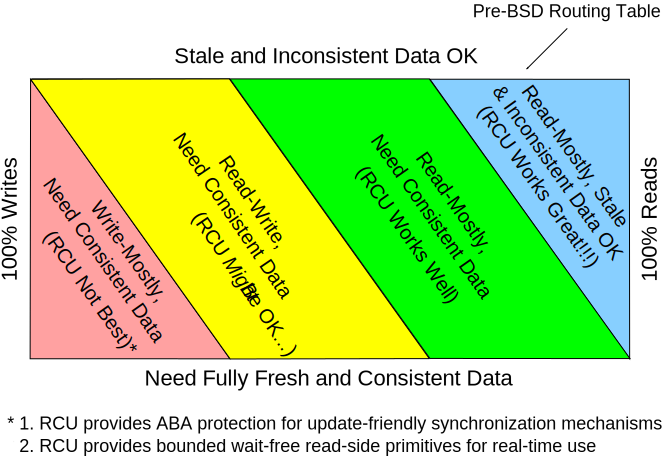
\includegraphics{defer/RCUApplicability}}
\end{center}
\caption{RCU Areas of Applicability}
\label{fig:defer:RCU Areas of Applicability}
\end{figure}

그전까지는,
Figure~\ref{fig:defer:RCU Areas of Applicability}
이 RCU 가 가장 도움되는 곳들에 대한 대략적인 규칙을 보입니다.

그림의 꼭대기의 파란 박스가 보이듯, RCU 는 낡고 비일관적인 데이터가 허용되고
읽기가 대부분인 데이터를 가지고 있을 때 가장 잘 동작합니다 (하지만 낡고
비일관적인 데이터에 대한 더 많은 정보를 위해 아래를 읽으세요).
리눅스 커널에서의 이런 케이스의 표준적 예제는 라우팅 테이블입니다.
라우팅 경로 업데이트가 인터넷을 통해 전파되기까지는 수초에서 심지어
분단위까지도 걸릴 수 있기 때문에, 시스템은 상당히 가끔 패킷들을 잘못된 방향으로
보낼 겁니다.
일부 패킷들을 잘못된 방향으로 보내는 작은 가능성을 수 밀리세컨드 동안 갖는 것은
결코 문제가 되지 않습니다.
\iffalse

In the meantime,
Figure~\ref{fig:defer:RCU Areas of Applicability}
shows some rough rules of thumb on where RCU is most helpful.

As shown in the blue box at the top of the figure, RCU works best if
you have read-mostly data where stale and inconsistent
data is permissible (but see below for more information on stale and
inconsistent data).
The canonical example of this case in the Linux kernel is routing tables.
Because it may have taken many seconds or even minutes for the
routing updates to propagate across Internet, the system
has been sending packets the wrong way for quite some time.
Having some small probability of continuing to send some of them the wrong
way for a few more milliseconds is almost never a problem.
\fi

일관적인 데이터가 필요한 읽기가 대부분인 워크로드라면, RCU 는 초록색의
``read-mostly, need consistent data'' 박스로 보인 것처럼 잘 동작합니다.
이런 케이스의 한가지 예는 리눅스 커널의 사용자 레벨 System-V 세마포어 ID 들부터
연관된 커널 내부 데이터 구조체들로의 매핑이 되겠습니다.
세마포어들은 그것들이 생성되고 사라지는 것보다 훨씬 더 빈번하게 사용되고,
따라서 이 매핑은 읽기가 대부분입니다.
하지만, 이미 삭제된 세마포어를 가지고 세마포어 오퍼레이션을 수행하는건 에러를
내기 쉬울겁니다.
이런 일관성의 필요는 커널 내 세마포어 데이터 구조체 내에 있는 락과 세마포어가
지워질 때 세워지는 ``deleted'' 플래그를 사용해 처리됩니다.
어떤 사용자 ID 가 ``deleted'' 플래그가 세워진 채 커널 내부 데이터 구조체에
매핑되면, 그 데이터 구조체는 무시되어서 그 사용자 ID 는 무효로 처리됩니다.
\iffalse

If you have a read-mostly workload where consistent data is required,
RCU works well, as shown by the green ``read-mostly, need consistent data''
box.
One example of this case is the Linux kernel's mapping from user-level
System-V semaphore IDs to the corresponding in-kernel data structures.
Semaphores tend to be used far more frequently than they are created
and destroyed, so this mapping is read-mostly.
However, it would be erroneous to perform a semaphore operation on
a semaphore that has already been deleted.
This need for consistency is handled by using the lock in the
in-kernel semaphore data structure, along with a ``deleted''
flag that is set when deleting a semaphore.
If a user ID maps to an in-kernel data structure with the
``deleted'' flag set, the data structure is ignored, so that
the user ID is flagged as invalid.
\fi

이런 방법은 읽기 쓰레드들이 세마포어 자체를 나타내는 데이터 구조체의 락을
잡아야 하게 하지만, 데이터 구조체의 매핑에는 락킹이 필요없게 해줍니다.
읽기 쓰레드들은 따라서 락을 사용하지 않고 ID 에서 데이터 구조체로의 매핑을 위해
사용된 트리를 횡단할 수 있는데, 이는 훨씬 향상된 성능, 확장성, 그리고 real-time
반응속도를 가져옵니다.
\iffalse

Although this requires that the readers acquire a lock for the
data structure representing the semaphore itself,
it allows them to dispense with locking for the
mapping data structure.
The readers therefore locklessly
traverse the tree used to map from ID to data structure,
which in turn greatly improves performance, scalability, and
real-time response.
\fi

노란색의 ``read-write' 박스로 보인 것처럼, RCU 는 일관적인 데이터가 필요한
read-write 워크로드에서도 유용하지만, 보통은 다른 동기화 도구들과 함게 사용될
때에 그렇습니다.
예를 들어, 최근의 리눅스 커널들의 디렉토리 엔트리 캐시는 시퀀스 락, CPU 별
락, 그리고 데이터 구조체별 락과 함께 RCU 를 사용해서 일반적인 경우의
pathname 들의 횡단을 락을 사용하지 않고 가능하게 합니다.
비록 RCU 가 이 read-write 케이스에는 많은 이득을 가져다 줄 수 있지만, 그런
사용은 읽기가 대부분인 경우에 비해 많은 경우 더 복잡합니다.
\iffalse

As indicated by the yellow ``read-write'' box, RCU can also be useful
for read-write
workloads where consistent data is required, although usually in
conjunction with a number of other synchronization primitives.
For example, the directory-entry cache in recent Linux kernels uses RCU in
conjunction with sequence locks, per-CPU locks, and per-data-structure
locks to allow lockless traversal of pathnames in the common case.
Although RCU can be very beneficial in this read-write case, such
use is often more complex than that of the read-mostly cases.
\fi

마지막으로, 그림 바닥의 빨간 박스가 나타내듯이, 일관적인 데이터를 필요로 하고
업데이트가 대부분인 워크로드는 일부 예외가 있긴
하지만~\cite{MathieuDesnoyers2012URCU} RCU 를 사용하기 좋은 곳이 아닐 확률이
높습니다.
또한,
Section~\ref{sec:defer:RCU is a Way of Providing Type-Safe Memory} 에서
이야기했듯, 리눅스 커널 내에서 \co{SLAB_DESTROY_BY_RCU} 슬랩 얼로케이터
플래그는 RCU 읽기 쓰레드들에게 type-safe 메모리를 제공하는데, 이는 non-blocking
동기화와 다른 락을 사용하지 않은 알고리즘들을 매우 간단하게 만들어줄 수
있습니다.
\iffalse

Finally, as indicated by the red box at the bottom of the figure,
update-mostly workloads requiring
consistent data are rarely good places to use RCU, though there are some
exceptions~\cite{MathieuDesnoyers2012URCU}.
In addition, as noted in
Section~\ref{sec:defer:RCU is a Way of Providing Type-Safe Memory},
within the Linux kernel, the \co{SLAB_DESTROY_BY_RCU}
slab-allocator flag provides type-safe memory to RCU readers, which can
greatly simplify non-blocking synchronization and other lockless
algorithms.
\fi

짧게 말해서, RCU 는 데이터 추가를 위한 publish-subscribe 메커니즘, 앞서 존재한
RCU 읽기 쓰레드들이 끝나길 기다리는 방법, 그리고 동시의 RCU 읽기 쓰레드들에
해를 끼치거나 지연시키지 않고 업데이트를 할 수 있도록 여러 버전들을 관리하는
규칙을 포함한 API 입니다.
이 RCU API 는 읽기가 대부분인 상황에 가장 잘 맞는데, 낡고 비일관적인 데이터가
허용되는 어플리케이션에서 특히 적합합니다.
\iffalse

In short, RCU is an API that includes a publish-subscribe mechanism for
adding new data, a way of waiting for pre-existing RCU readers to finish,
and a discipline of maintaining multiple versions to allow updates to
avoid harming or unduly delaying concurrent RCU readers.
This RCU API is best suited for read-mostly situations, especially if
stale and inconsistent data can be tolerated by the application.
\fi
